\documentclass[report, 11pt, twoside]{report}

\usepackage{fullpage}
\usepackage[utf8]{inputenc}
\usepackage[T1]{fontenc}
\usepackage[french]{babel} 
\usepackage{graphicx}
%\usepackage{url} %pour écrire des adresses cliquables
\usepackage{lmodern} %pour changer le pack de police
%\usepackage[top=5cm, bottom=5cm, left=6cm, right=3cm]{geometry} %pour les marges
\usepackage[usenames, dvipsnames]{color}
\usepackage{listings}
\usepackage{hyperref} %pour un fichier PDF  interactif
\usepackage[final]{pdfpages}
\usepackage[table]{xcolor}
\usepackage{acronym}

\graphicspath{{images/}}

\acrodef{SGBD}{système de gestion de base de données}

\pdfcompresslevel=9

\hypersetup{
	backref=true, %permet d'ajouter des liens dans...
	pagebackref=true, %...les bibliographies
	hyperindex=true, %ajoute des liens dans les index.
	colorlinks=true, %colorise les liens
	breaklinks=true, %permet le retour à la ligne dans les liens trop longs
	urlcolor=blue, %couleur des hyperliens
	linkcolor=blue, %couleur des liens internes
	bookmarks=true, %créé des signets pour Acrobat
	bookmarksopen=true,%si les signets Acrobat sont créés,
	%les afficher complètement.
	%pdftitle={Mon fabuleux livre}, %informations apparaissant dans
	%pdfauthor={Pejvan BEIGUI},%dans les informations du document
	%pdfsubject={Mac OS X}%sous Acrobat.
}


\lstdefinestyle{php}{
	language=PHP,
	caption={PHP},
	basicstyle= \footnotesize,
	tabsize=4,
	showspaces=false,
	showstringspaces=false,
	showtabs=false,
	breaklines=true,
	breakautoindent=true,
	identifierstyle=\color{RoyalBlue},
	commentstyle=\color{LimeGreen},
	keywordstyle=\color{Black},
	stringstyle=\color{OrangeRed},
	backgroundcolor=\color{white},
	numbers=left
}

\begin{document}

\title{Carcajou}
\author{\textsc{Martin Desharnais} \\ \textsc{Samuel Milette-Lacombe} \\ \textsc{Marc-André Destrempes}}
\date{\today}

\maketitle

\begin{abstract}
Ce document contient la documentation du projet de médiathèque (nom de code «~Carcajou~») conçu pour le département de musique du CEGEP de Trois-Rivières.
\end{abstract}

\newpage
\tableofcontents
\newpage

%%%%%%%%%%%%%%%%%%%%%%%%%%%%%%%%%%%%%%%%%%%%%%%%%%
\chapter{Spécifications fonctionnelles}
%%%%%%%%%%%%%%%%%%%%%%%%%%%%%%%%%%%%%%%%%%%%%%%%%%


\section{Médias}

Nous avons décidé de centraliser un certain nombre d'informations communes à tous les articles pouvant faire partie de la médiathèque, comme le titre ou le numéro de référence, sous l'identité de média. Ainsi, tous les articles de la médiathèque sont des médias et partagent un certain nombre de propriétés. Par la suite, ceux-ci sont subdivisés en médias audios, vidéos et imprimés où chaque subdivision contient un certain nombre d'informations unique à sa catégorie.

Au niveau de la base de données, cette situation se traduit par une table \texttt{medias} qui contient un enregistrement correspondant à tous les médias de la médiathèque ainsi que des tables enfants contenant les informations plus précises de chaque type.

Les informations propres aux médias imprimés se trouvent dans la table \texttt{imprimes}.

Les médias audio et vidéos sont un cas à part, car nous nous sommes aperçus que ceux-ci étaient extrêmement semblables. Les quelques propriétés qui les distinguaient pouvaient très bien s'appliquer l'un à l'autre. Nous avons donc décidé, à l'interne, de les regrouper dans la table \texttt{audios\_videos}.

\begin{table}[htbp]
	\caption{medias}
	\label{tab:sf-medias}
	\begin{center}
		\begin{tabular}{|c|l|c|}
			\hline
			ID & titre                                 & annee\_publication \\
			\hline
			1  & L'expédition                          & 2008 \\
			2  & La communauté de l'anneau             & 1972 \\
			3  & La communauté de l'anneau             & 2005 \\
			4  & Indiana Jones et la dernière croisade & 1987 \\
			\hline
		\end{tabular}
	\end{center}
\end{table}

\begin{table}[h!tbp]
	\caption{audios\_videos}
	\label{tab:sf-audios-videos}
	\begin{center}
		\begin{tabular}{|c|c|l|}
			\hline
			ID & exID & nationalite \\
			\hline
			1  & 1    & Canadienne \\
			2  & 4    & Américaine \\
			\hline
		\end{tabular}
	\end{center}
\end{table}

\begin{table}[htbp]
	\caption{imprimes}
	\label{tab:sf-imprimes}
	\begin{center}
		\begin{tabular}{|c|c|l|}
			\hline
			ID & exID & collection \\
			\hline
			1  & 2    & Le seigneur des anneaux \\
			2  & 3    & Le seigneur des anneaux \\
			\hline
		\end{tabular}
	\end{center}
\end{table}

Ainsi, pour effectuer une interrogation à la base de données concernant l'ensemble des médias, il suffit d'interroger la table \texttt{medias} qui contient les informations communes à tous les médias. Si nous voulons des informations plus précises sur un média audio, il suffit de joindre les tables \texttt{medias} et \texttt{audios\_videos} selon l'\texttt{ID} du premier et l'\texttt{exID} du second.

Nous pouvons toujours être surs que, pour chaque enregistrement de la table \texttt{media}, il y aura toujours, selon le type, un enregistrement correspondant dans la table \texttt{audios\_videos} ou bien dans la table \texttt{imprimes}.

Dans l'exemple des tableaux \ref{tab:sf-medias}, \ref{tab:sf-audios-videos} et \ref{tab:sf-imprimes}, nous voyons que le CD \emph{l'expédition}, paru en 2008, est de nationalité canadienne alors que le livre \emph{La communauté de l'anneau}, paru en 1972, appartient à la collection \emph{Le seigneur des anneaux}. Ce sont tous deux des médias, mais les informations supplémentaires de chacun sont dans la table correspondant à leur type.

Nous pouvons aussi constater qu'il y a deux médias portant le même titre, mais ayant une date de publication différente. Il s'agit là d'une réédition et puisque certaines informations changent d'une édition à l'autre, un nouveau média a été créé pour la représenter.

\begin{table}[htbp]
	\caption{exemplaires\_medias}
	\label{tab:sf-exemplaires-medias}
	\begin{center}
		\begin{tabular}{|c|c|l|}
			\hline
			ID & exID & reference \\
			\hline
			1  & 1    & CD-00001 \\
			2  & 1    & CD-00002 \\
			3  & 2    & ROM-00003 \\
			4  & 3    & ROM-00004 \\
			5  & 4    & VHS-00005 \\
			\hline
		\end{tabular}
	\end{center}
\end{table}

Il peut aussi arriver que nous disposions de plusieurs copies identiques d'un même média. Dans ce cas, nous pouvons simplement ajouter un exemplaire à un média déjà présent dans la base de données. Dans le tableau \ref{tab:sf-exemplaires-medias}, nous pouvons voir que nous possédons deux exemplaires de l'album \emph{l'expédition} alors que nous ne possédons qu'un seul exemplaire des autres médias. Puisque ce sont des objets distincts, les deux albums ont un numéro de référence différent afin de permettre de les différencier.

L'analyse nous a révélé que certains médias ne peuvent être empruntés que par certains groupes d'utilisateurs alors que d'autres sont disponibles uniquement pour consultation sur place.

Pour représenter cette situation, nous avons décidé que chaque média contiendra la liste des groupes habilités à l'emprunter. Si aucun groupe n'est défini, cela signifie que personne ne peut l'emprunter et qu'il est disponible en consultation sur place seulement.

\subsection{Suggestions}
Les utilisateurs du site ont la possibilité d'émettre une suggestion d'achat de nouveaux médias. Un formulaire les invite à entrer le titre, l'artiste ainsi que le type de support du média qu'ils comptent suggérer. Ils ont aussi la possibilité d'ajouter un commentaire si des informations supplémentaires sont nécessaires.

Le champ permettant d'entrer l'artiste devra être lié à une liste de suggestions permettant à l'utilisateur de sélectionner un artiste déjà présent dans le système. Pour plus d'informations sur les listes de suggestions, voir la section \ref{sec:recherche-avancée} sur la recherche avancée. Le champ contenant l'artiste ne peut être une simple liste déroulante statique puisque nous désirons laisser à l'utilisateur la possibilité de suggérer un média appartenant à un nouvel artiste.

\section{Recherche}

Des fonctions de recherche simple et avancée sont un élément essentiel pour un système de médiathèque. Le nôtre n'en fait pas exception puisqu'il offre un module de recherche évolué et des possibilités de raffinement sans limites. Nous avons voulu créer un système de recherche nécessitant un temps d'apprentissage quasi nul. Pour cela, nous avons joint quelques particularités aux fonctions de recherche de base. Voici la liste des éléments assurant une facilité de recherche et une bonne navigabilité des résultats correspondants à cette recherche.

\begin{itemize}
	\item Fil d'Ariane vertical permettant de raffiner les résultats de recherche;
	\item Mode «~Parcourir~» permettant de parcourir tous les médias;
	\item Recherche simple de médias;
	\item Recherche avancée de médias;
\end{itemize}

\subsection{Fil d'Ariane vertical}
Un fil d'Ariane est un composant web d'aide à la navigation dans les pages d'un site web. Un fil d'Ariane horizontal standard est sous la forme de signalisation de la localisation du lecteur dans un document. Il permet d'indiquer à l'utilisateur où il se situe dans une page web et offre la possibilité de revenir à la section qu'il désire.  Dans le cas de Carcajou, c'est un fil d'Ariane vertical qui est utilisé. Au lieu de nous afficher notre position dans un site web sous forme d'arborescence, il nous permet de naviguer par critères dans les résultats de recherche. On pourra donc l'utiliser pour raffiner une recherche de médias. Pour une recherche donnée, une liste de valeurs regroupées par critères sera affichée et l'on pourra donc cliquer sur ces valeurs pour raffiner sa recherche. 

\begin{figure}[htbp]
	\begin{center}
		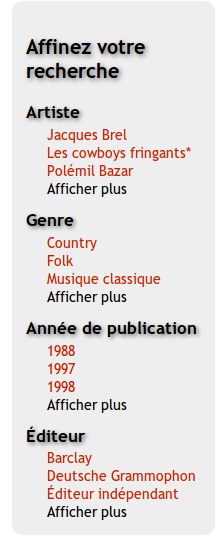
\includegraphics[scale=0.5]{captures_ecran/exemple_fil_darianne.png}
	\end{center}
	\caption{Exemple de fil d'Ariane vertical}
\end{figure}

Plus la recherche sera raffinée, moins le fil d'Ariane sera rempli puisque la recherche devient plus spécifique et de moins en moins de valeurs d'attribut seront applicables à la recherche. Par exemple, si le niveau de raffinement de la recherche retourne uniquement deux résultats et que ces médias ont le même attribut « genre », il est évident que ce critère ne sera pas affiché dans le fil d'Ariane. Lorsqu’aucune possibilité de raffinement supplémentaire n’est disponible pour les résultats affichés. 

\begin{figure}[htbp]
	\begin{center}
		
\includegraphics[scale=0.5]{captures_ecran/recherche_rafinnee_au_max.png}
	\end{center}
	\caption{Fil d'Ariane lorsque raffiné au maximum}
\end{figure}

Pour ajouter à l'ergonomie déjà présente dans le fil d'Ariane, nous avons établi que s'il y avait plus de trois suggestions de valeurs pour un critère, une entrée de liste "Afficher plus" serait affichée pour développer les valeurs supplémentaires. La page est donc moins surchargée. Il est à noter que cette fonction n'est disponible que sur un navigateur ayant le JavaScript activé. La désactivation du JavaScript n'amène pas de problèmes en tant que tels. Les valeurs des critères seront tout simplement affichées dans leur ensemble sans possibilité de cacher X résultats.

\subsection{Parcourir}
Le mode « Parcourir » est tout simplement l'exécution d'une recherche n'ayant aucun critère spécifique. Tous les médias sont donc affichés. Une surcharge de résultats sur la page est évitée avec l'utilisation du système de pagination affichant 5 résultats par page. Pour raffiner les résultats de la recherche, on utilise le fil d'Ariane vertical décrit précédemment.

\subsection{Recherche simple}
Accessible à partir de la barre de navigation principale, la recherche simple permet à partir d'un mot clé d'effectuer une recherche sur tous les médias. Seuls les médias satisfaisant le mot clé évoqué seront affichés. Pour cela, tous les champs sont parcourus pour rechercher une correspondance à ce mot clé en ignorant la casse. Par exemple, une recherche avec le mot « cowboy » pourrait autant retourner un média de l'artiste « Les cowboys fringants » qu'un média contenant la chanson «~Bye Bye Mon Cowboy~».

\begin{figure}[htbp]
	\begin{center}
		
\includegraphics[scale=0.5]{captures_ecran/barre_recherche_simple.png}
	\end{center}
	\caption{Barre de recherche simple}
\end{figure}

\subsection{Recherche avancée}
\label{sec:recherche-avancée}
La recherche avancée permet de faire une recherche très spécifique. On peut y sélectionner tous les critères de recherche possible et sans limites de nombre. On peut sélectionner les opérateurs logiques (et, ou, etc.) et les opérateurs de comparaison (contient, égale, etc.). On pourrait donc effectuer une recherche comme celle-ci: Titre du média contenant « Indiana Jones» et année de publication plus grande que 1988.

\begin{figure}[htbp]
	\begin{center}
		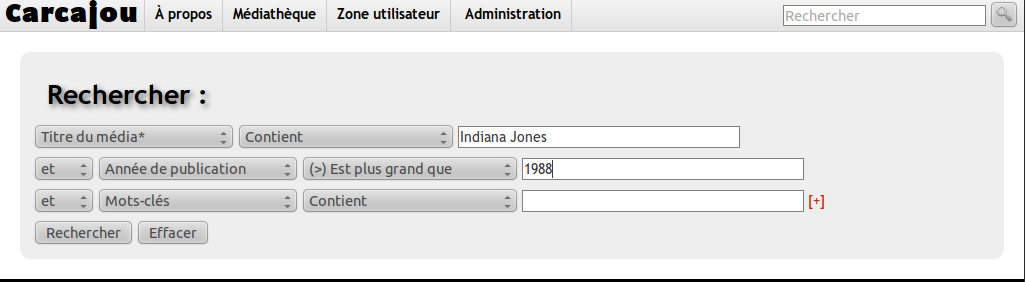
\includegraphics[scale=0.5]{captures_ecran/exemple_recherche_avancee.png}
	\end{center}
	\caption{Exemple de recherche avancée}
\end{figure}

Lors de la sélection d'un critère d'une recherche, une liste de suggestions est automatiquement liée au champ texte. Dès que l'on tape une série de lettres, une liste de valeurs contenant ce groupe de lettres s'affichera.  Cet ajout rend la recherche avancée beaucoup plus conviviale. Cette fonctionnalité utilise la balise «~\href{http://www.w3schools.com/html5/tag_datalist.asp}{datalist}~» qui est disponible uniquement sur des navigateurs supportant cette balise Html 5.

\begin{figure}[htbp]
	\begin{center}
		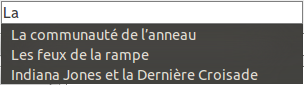
\includegraphics[scale=0.5]{exempleDatalist.png}
	\end{center}
	\caption{Exemple de suggestions à partir d'une datalist}
\end{figure}

Il est aussi possible d'ajouter autant de critères de recherches que l'on désire. Pour cela, le JavaScript a été utilisé pour interagir dynamiquement avec le DOM de la page. Des effets visuels de disparation et d'apparition ont même été ajoutés pour une ergonomie plus dynamique.

\begin{figure}[htbp]
	\begin{center}
		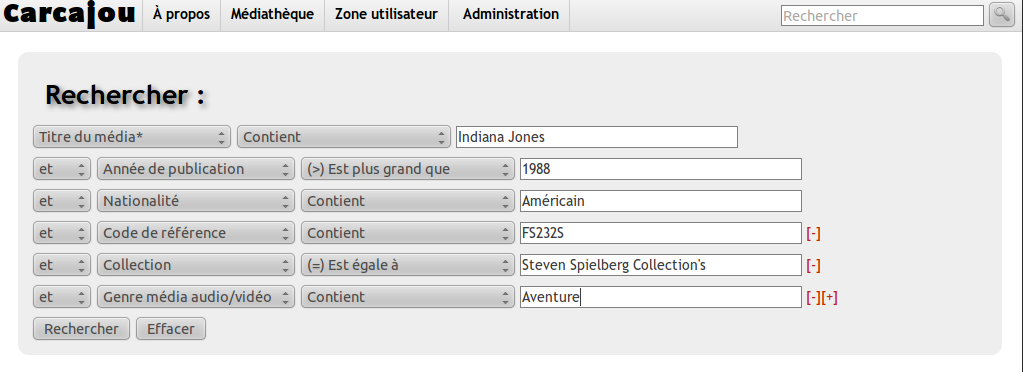
\includegraphics[scale=0.5]{captures_ecran/exemple_recherche_avancee2.png}
	\end{center}
	\caption{Ajout d'un nombre personnalisé de critères}
\end{figure}

\section{Gestion des utilisateurs}

Suite à l'analyse du projet, nous avons relevé qu'il y a, principalement, quatre groupes d'utilisateurs à gérer~:
\begin{itemize}
	\item Les \emph{administrateurs} du système qui ont tous les droits;
	\item Les \emph{commis} qui sont chargé d'entrer les emprunts, les réservations et les nouvelles acquisitions;
	\item Les \emph{étudiants} qui ont le droit d'effectuer des réservations, mais dépendent d'un commis pour emprunter et retourner un média;
	\item Les \emph{enseignants} du département qui n'ont pas à passer par le commis pour effectuer un emprunt ou un retour à leur nom.
\end{itemize}

\subsection{Utilisateurs}
Chaque personne souhaitant bénéficier des services de la médiathèque doit avoir un compte utilisateur identifié par nom d'utilisateur\footnote{Actuellement, nous utilisons le matricule comme nom d'utilisateur.} ainsi qu'un mot de passe. À moins que, lors de la programmation, les informations nécessaires soient disponibles, ces identifiants sont dissociés des noms d'utilisateurs et mots de passe utilisés pour accéder aux services LÉA et aux ordinateurs du cégep de Trois-Rivières. Cependant, rien n'empêche les utilisateurs de choisir le même mot de passe pour les deux systèmes.

Toutes les informations sur un utilisateur sont stockées dans la table \texttt{utilisateurs}. Il est important de noter que les informations personnelles de l'utilisateur doivent en tout temps rester accessibles au moins de personnes possible\footnote{Ceci est un exemple évident de l'application du «~\href{http://en.wikipedia.org/wiki/Principle_of_least_privilege}{Principle of least privilege}~».}. Ceci est possible grâce au système de gestion des droits qui permet de donner le droit en lecture à ces informations uniquement à certains groupes (e.g.\ \emph{Administrateurs} et \emph{Commis}).

Pour plus d'informations sur la gestion des droits et la sécurité, voir la section \ref{sec:sécurité} sur la sécurité à la page \pageref{sec:sécurité}.

Certaines informations, comme le mot de passe de l'utilisateur, doivent rester totalement inconnues de tous, excepté de l'utilisateur lui-même. Pour ce faire, ces informations devront être cryptées avant d'être enregistrées dans la base de données. Dans le cas où un utilisateur perde sont mot de passe, la seule solution consiste à le réinitialiser à une valeur par défaut et à demander à l'utilisateur d'en définir un nouveau.

\subsection{Groupes}
Les groupes servent à effectuer une distinction entre les différents utilisateurs et à leur attribuer des droits correspondant à leur statut dans le département. Plutôt que de tenter de prédire tous les besoins de hiérarchisation des utilisateurs dont le département de musique aura besoin dans le futur, nous avons pris la décision de rendre la gestion des groupes accessible aux utilisateurs. Ainsi, dans cinq ans, un administrateur pourrait créer un nouveau groupe avec des droits spécifiques pour représenter une nouvelle situation, comme l'arrivée d'enseignants stagiaires.

Pour plus d'informations sur la gestion des groupes et la sécurité, voir la section \ref{sec:sécurité} sur la sécurité à la page \pageref{sec:sécurité}.

\section{Zone utilisateur}
La zone utilisateur permet à l'utilisateur actuellement connecté d'accéder à des informations concernant son utilisation de la médiathèque.

\subsection{Mes réservations}
La page «~Mes réservations~» permet à l'utilisateur de consulter la liste des réservations qu'il a actuellement. Celles-ci sont affichées dans un tableau où il est possible de définir l'information de tri simplement en cliquant sur l'en-tête de la colonne. De plus, un lien offre à l'utilisateur la possibilité de supprimer une réservation. Si le JavaScript est activé, une invite de confirmation demande à l'utilisateur de confirmer qu'il désire bien supprimer la réservation. Dans le cas où le JavaScript est désactivé, la réservation est supprimée sans demander de confirmation.

Une fois celle-ci supprimée, un courriel doit être envoyé à l'utilisateur afin de lui confirmer la suppression de sa réservation.

L'utilisateur peut consulter la fiche détaillée du média en cliquant sur son titre dans le tableau.

\subsection{Mes emprunts en cours}
La page «~Mes emprunts en cours~» permet à l'utilisateur de consulter la liste des médias qu'il a actuellement en sa possession. Ceux-ci sont affichés dans un tableau où il est possible de définir l'information de tri simplement en cliquant sur l'en-tête de la colonne. De plus, un lien offre à l'utilisateur la possibilité de demander un renouvellement d'un emprunt.

L'utilisateur peut consulter la fiche détaillée du média en cliquant sur son titre dans le tableau.

\subsection{Mon historique d'emprunts}

La page «~Mon historique d'emprunts~» permet à l'utilisateur de consulter la liste des emprunts qu'il a effectués par le passé. Ceux-ci sont affichés dans un tableau où il est possible de définir l'information de tri simplement en cliquant sur l'en-tête de la colonne.

L'utilisateur peut consulter la fiche détaillée du média en cliquant sur son titre dans le tableau.

\section{Administration}
La zone d'administration permet aux utilisateurs possédant les droits requis d'effectuer des emprunts, des retours, des rapports, de générer des codes QR, de faire la gestion des groupes, des utilisateurs et des tables de pilotages.

\subsection{Emprunt et retour}
Les pages «~Emprunt~» et «~Retour~» permettent, aux personnes qui ont les droits requis, d'entrer des emprunts et retours dans la base de données. Pour effectuer un emprunt ou retour, la personne qui veut emprunter présente sa carte. À partir d'un lecteur de QR code on numérise le code et celui rempli automatiquement le champ désigné. On effectue la même opération lorsqu'il s'agit d'ajouter les médias. Ces deux opérations peuvent aussi s'effectuer à la main, c'est-à-dire entrer les codes manuellement. Pour supprimer un média de la liste lors d'une erreur, la personne n'a qu'à entrer le numéro de référence à nouveau et appuyer sur le +. Pour les emprunts, les dates disponibles vont changer selon les réservations et les disponibilités du commis. Les retours n'ont pas besoin de dates.

\subsection{Générer code QR}
À partir du générateur de code QR, l'usagé n'a qu'à entrer le texte qu'il veut et le code QR correspondant sera généré. Dans le contexte présent, l'utilité de ces codes est de permettre l'identification des médias sans commettre d'erreurs. Ces codes peuvent contenir le texte désiré. Ainsi, le code de référencement maison peut toujours être utilisé. Si nous voulons pousser plus loin encore, les codes QR pourront être utilisés pour la fabrication de cartes qui seront remises aux usagés pour assurer un meilleur contrôle de ce qui entre et sort.

\begin{figure}[htbp]
	\begin{center}
		
\includegraphics[scale=0.5]{qr.png}
	\end{center}
	\caption{Exemple de code QR}
\end{figure}

\subsection{Tables de pilotages}
\label{sec:tables_de_pilotage}
De nombreuses tables de la base de données sont basées sur le concept de table de pilotage. Celles-ci sont des tables qui servent à définir une liste de valeurs possibles pour une colonne d'une ou plusieurs autres tables. Par exemple, la table \texttt{medias} offre le champ \texttt{maison\_edition} qui permet d'identifier la maison d'édition d'un média donné. Plutôt que de fournir un champ texte de 50 à 75 caractères de long et de devoir réécrire le nom de la maison d'édition pour chaque enregistrement, nous avons créé la table \texttt{maisons\_edition} qui contient la liste de toutes les maisons d'édition utilisables par le système. La colonne \texttt{medias.maison\_edition} ne contient donc qu'une clé étrangère pointant sur l'enregistrement correspondant de sa table de pilotage.

De plus, nous avons ajouté une colonne \texttt{inactif} à toutes les tables de pilotage afin que l'utilisateur puisse définir une valeur comme n'étant plus utilisable dans le futur. D'aucun pourrais suggérer de simplement supprimer cette valeur, mais un bon \ac{SGBD} appliquant l'intégrité référentielle refusera une telle opération si ne serait-ce qu'une clé étrangère pointe sur l'enregistrement. Nous pourrions très bien supprimer toutes les clés étrangères avant d'effectuer la suppression, mais, en y réfléchissant bien, nous ne souhaitons pas faire disparaitre toute trace de la valeur, nous souhaitons simplement qu'elle ne puisse plus être utilisée à l'avenir. En définissant un champ inactif, nous permettons à l'utilisateur de bloquer l'utilisation d'une valeur pour le futur tout en laissant les enregistrements l'utilisant déjà intacts.

Dans le contexte d'un formulaire permettant d'entrer des médias, cette relation se traduit par une liste déroulante, remplie de toutes les valeurs non inactives, où il suffit de choisir une valeur parmi celles proposées.

\begin{figure}[htbp]
	\begin{center}
		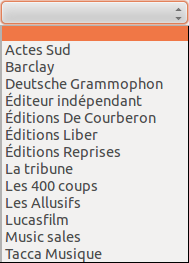
\includegraphics[scale=0.5]{exempleListeDeroulante.png}
	\end{center}
	\caption{Exemple de liste déroulante}
\end{figure}

Cette technique offre de nombreux avantages dont voici une liste non exhaustive~:
\begin{itemize}
	\item Possibilité de filtrer les valeurs acceptables pour un champ;
	\item Possibilité de définir une valeur comme n'étant plus disponible pour utilisation future, mais restant valide pour les utilisations passées;
	\item Possibilité d'éviter tout risque de dédoublement de valeurs suite à des fautes d'orthographes\footnote{La seule possibilité de dédoublement des valeurs est si la personne chargée de gérer les tables de pilotages écrit deux fois la même valeur avec une orthographe différente (e.g.\ Trois-Rivières et trois-rivieres).}.
	\item Possibilité de mettre à jour instantanément la valeur d'une option pour tous les enregistrements l'utilisant en modifiant simplement sa valeur dans la table de pilotage.
	\item Poid de la base de données réduit puisqu'il est moins lourd de définir de nombreuses clés étrangères que de répéter de nombreuses fois la même chaine de caractères.
	\item Possibilité de ne donner les droits de modification à la table de pilotage qu'à certains groupes d'utilisateurs.
\end{itemize}

La zone d'administration permet à l'utilisateur d'ajouter, modifier et supprimer des données de nombreuses tables de pilotages. La page de modification se présente sous forme de tableau où il est possible de définir l'information de tri simplement en cliquant sur l'en-tête de la colonne correspondante et où la première ligne sert à entrer une nouvelle valeur. Un bouton permet de supprimer une valeur, mais, comme dit précédemment, la suppression ne doit être acceptée que si aucune clé étrangère n'est définie sur cet enregistrement.

C'est l'une des rares pages du site qui est totalement dépendante du JavaScript et requiert donc qu'il soit activé sur le navigateur des utilisateurs souhaitant modifier les tables de pilotages.

Comme la taille d'une table de pilotage peut devenir assez grande, et que tous les enregistrements apparaissent dans le formulaire, nous avons développé un système permettant aux futurs programmeurs de mettre facilement à jour la table. Sans cette technique, il aurait toujours fallu mettre à jour tous les enregistrements, ajouter tous ceux ne figurant pas dans la nouvelle liste et supprimer tous ceux n'y figurant plus. Toutes ces opérations auraient été très couteuses en ressources et très difficiles à mettre en place.

Pour palier à ces problèmes, nous avons ajouté une colonne invisible dans le formulaire qui a pour nom \texttt{row\_state}. Celle-ci contient un nombre qui ne peut avoir que quatre valeurs~:

\begin{table}[htbp]
	\caption{Valeurs possibles de la colonne \texttt{row\_state}}
	\begin{center}
		\begin{tabular}{|c|l|}
			\hline
			Valeur & Significaton \\
			\hline
			1      & Unchanged \\
			2      & Added \\
			3      & Deleted \\
			4      & Modified \\
			\hline
		\end{tabular}
	\end{center}
\end{table}

La valeur de la colonne est modifiée en JavaScript selon les modifications faites à chaque enregistrement. Lorsque le formulaire est envoyé au serveur, le programmeur sait qu'il n'a rien à faire avec les enregistrements dont la \texttt{row\_state} est à 1, qu'il doit faire une requête \texttt{INSERT} lorsqu'elle est à 2, qu'il doit faire une requête \texttt{DELETE} lorsqu'elle est à 3 et une requête \texttt{UPDATE} lorsqu'elle est à 4.

Comme les tables de pilotages sont nombreuses et que leur formulaire de modification est très semblable, nous avons décidé que, plutôt que de faire une page séparée par table de pilotage, une seule page se permettrait de toutes les modifier. Tous les hyperliens pointent donc vers la même page et se contentent de passer en paramètre la table qui doit être modifiée. La page se connecte alors à la base de données afin de l'interroger sur la structure de la table en question et génère alors dynamiquement un formulaire contenant toutes les colonnes celle-ci.

Cette façon de faire permet de s'assurer que le formulaire sera toujours parfaitement à jour avec la structure de la table dans la base de données et permet aussi d'ajouter de nouvelles tables de pilotage très facilement et très rapidement puisqu'il n'y a pas de nouveau formulaire à créer.

\subsection{Réservations en cours}
La page «~Réservations en cours~» permet à l'utilisateur de consulter la liste de toutes les réservations du système. Celles-ci sont affichées dans un tableau où il est possible de définir l'information de tri simplement en cliquant sur l'en-tête de la colonne. L'utilisateur a aussi la possibilité de supprimer une réservation. Une invite de confirmation lui est alors affichée et un courriel est envoyé à l'utilisateur à l'origine de la réservation pour lui indiquer que celle-ci a été supprimée.

L'utilisateur peut consulter la fiche détaillée du média en cliquant sur son titre dans le tableau et la fiche détaillée de l'utilisateur en cliquant sur son nom.

\subsection{Emprunts en cours}
La page «~Emprunts en cours~» permet à l'utilisateur de consulter la liste de tous les médias qui sont actuellement empruntés. Ceux-ci sont affichés dans un tableau où il est possible de définir l'information de tri simplement en cliquant sur l'en-tête de la colonne.

L'utilisateur peut consulter la fiche détaillée du média en cliquant sur son titre dans le tableau et la fiche détaillée de l'utilisateur en cliquant sur son nom.

\subsection{Historique des emprunts}
La page «~Historique des emprunts~» permet à l'utilisateur de consulter l'historique de tous les emprunts du système. Ceux-ci sont affichés dans un tableau où il est possible de définir l'information de tri simplement en cliquant sur l'en-tête de la colonne.

L'utilisateur peut consulter la fiche détaillée du média en cliquant sur son titre dans le tableau et la fiche détaillée de l'utilisateur en cliquant sur son nom.

\subsection{Gestion des utilisateurs}
La page de gestion des utilisateurs permet~:
\begin{enumerate}
	\item De visualiser tous les utilisateurs ou bien seulement ceux d'un groupe donné;
	\item D'ajouter un nouvel utilisateur;
	\item D'importer plusieurs nouveaux utilisateurs;
	\item De modifier un utilisateur;
	\item De supprimer un utilisateur.
\end{enumerate}

Les utilisateurs sont affichés dans un tableau où il est possible de définir l'information de tri simplement en cliquant sur l'en-tête de la colonne. Par défaut, tous les utilisateurs sont affichés. Si l'on souhaite afficher uniquement les utilisateurs appartenant à un groupe donné, il suffit de sélectionner ce groupe dans la liste déroulante située dans le coin supérieur droit de la page.

L'ajout d'un utilisateur nous apporte dans un formulaire permettant d'entrer les informations de celui-ci alors que la modification nous amène au même formulaire, mais avec les informations préremplies de l'utilisateur à modifier. C'est à partir de ce formulaire qu'une liste de sélection multiple nous permet de sélection tous les groupes auxquels appartient l'utilisateur\footnote{Voir la section \ref{sec:sécurité}, à la page \pageref{sec:sécurité}, pour plus d'informations sur les groupes et la sécurité.}.

Pour ce qui est de la suppression, une invite de confirmation demande à l'utilisateur de confirmer qu'il désire bien supprimer l'utilisateur.

L'importation, quant à elle, se résume actuellement à un hyperlien qui ne mène nulle part puisqu'il ne nous a pas été dit comment allait se passer la synchronisation des utilisateurs avec les élèves du département de musique. Nous avons fait comme hypothèse que l'importation se fera à partir d'un fichier XML qui contiendra la liste des nouveaux utilisateurs. Ceux qui programmeront le système devront donc se charger de mettre en place un système d'importation qui se mettra en action lors du clique sur ledit hyperlien.

\subsection{Gestion des groupes}
À l'heure actuelle, la gestion des groupes se présente de la même façon que la gestion d'une table de pilotage\footnote{Voir la section \ref{sec:tables_de_pilotage}, à la page \pageref{sec:tables_de_pilotage}, pour plus d'informations sur les tables de pilotages.}.

Lorsque le système sera implémenté, les programmeurs auront le choix d'offrir ou non au client la possibilité de modifier les droits de groupes. Puisque des droits de groupes mal configurés risquent d'amener des failles de sécurités, le client préférera peut-être demander au département d'informatique chaque fois que de telles manipulations seront nécessaires.

\section{Rapports}

\subsection{Rapport sur les médias audios}
La page «~Rapport~» permet, aux personnes qui ont les droits requis, de générer un rapport sur les médias selon le genre sélectionné. Le résultat du rapport est présenté dans un tableau simple et efficace qui est trié par ordre de code de référence, par titre et par année de publication. Le but de pouvoir faire des rapports est de générer une liste de ce que l'on cherche rapidement et efficacement, le tout sans erreurs, pour accélérer le travail par la suite. D'autres rapports du genre pourront être ajoutés sur demande.

\section{Pages d'information}

Nous avons intégré une section «~À propos~» qui les sections suivantes~:
\begin{itemize}
	\item À propos de la médiathèque;
	\item À propos du département de musique;
	\item À propos des heures d'ouverture;
	\item À propos de la règlementation.
\end{itemize}

Ces pages permettront de publier des informations concernant la médiathèque et le département de musique comme. Ce sera l'endroit idéal pour parler de l'évolution du département de musique et de leur médiathèque ainsi que pour expliquer le fonctionnement du site.

%%%%%%%%%%%%%%%%%%%%%%%%%%%%%%%%%%%%%%%%%%%%%%%%%%
\chapter{Architecture du système}
%%%%%%%%%%%%%%%%%%%%%%%%%%%%%%%%%%%%%%%%%%%%%%%%%%

\section{Charte graphique}

\subsection{Introduction}

Le site doit véhiculer l'image universelle de la musique. Nous avons donc choisie un thème graphique près du noir sur blanc pour s'apparenter aux touches d'un piano qui est un des instruments le plus représentatifs de l'image qu'ont le peuple Nord-Américain de la musique. Pour cela, une charte graphique a été définie. Elle dégage une ambiance sobre et pratique. De plus, cette charte respecte le sérieux, l'élégance et la fierté des institutions de musique, tel un orchestre symphonique constitué de musiciens vêtus de vestons cravates.

\subsection{Maquette}

Toutes les pages sont construites sur la base du modèle suivant :

\begin{enumerate}
	\item Bandeau
	\item Fil d'Ariane vertical (n'apparais cependant que dans certaines pages)
	\item Contenu de la page
	\item Pied de page
\end{enumerate}

\begin{figure}[h!tbp]
	\begin{center}
		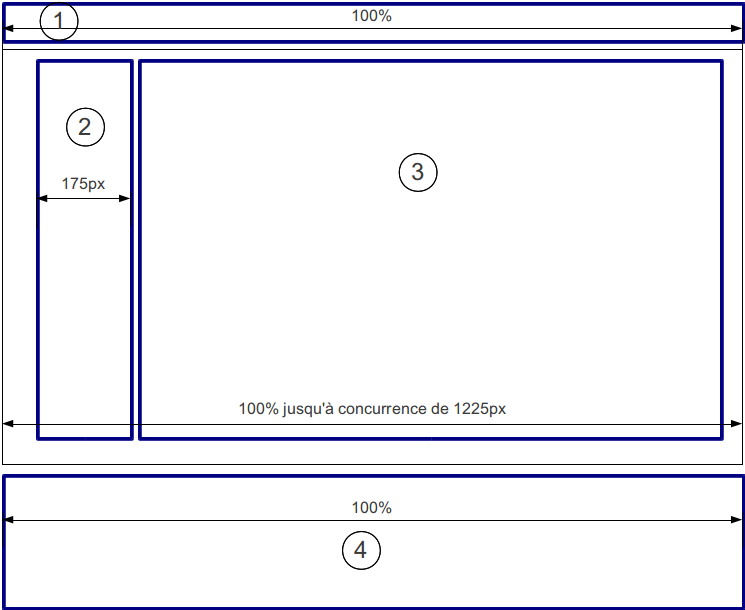
\includegraphics[scale=0.59]{maquetteImage.png}
	\end{center}
	\caption{Maquette générale du site}
\end{figure}

\subsubsection{Bandeau (1)}

Le bandeau est constitué des éléments suivants:
\begin{description}
	\item[Sigle Carcajou] Le sigle Carcajou est en fait le logo du site et est toujours situé dans le coin supérieur gauche. Par contre, ce n'est pas une image, mais bien un mot mise en forme en CSS. Ce sigle permet, en tout temps, de revenir sur la page d'accueil. Le sigle du site utilise la police MegalopolisExtra-Webfont.
	\item[Menus déroulants]À la droite du sigle se retrouve le menu principal incluant des menus déroulants permettant de se déplacer dans les sections du site. Les entrées de menu sont les suivantes:
		\begin{itemize}
			\item À propos
			\begin{itemize}
				\item De la médiathèque
				\item Du département de musique
				\item Des heures d'ouverture
				\item De la règlementation
			\end{itemize}
		\end{itemize}
		\begin{itemize}
			\item Médiathèque
			\begin{itemize}
				\item Recherche avancée
				\item Parcourir
				\item Suggestions
			\end{itemize}
		\end{itemize}
		\begin{itemize}
			\item Zone utilisateur (lorsque non connecté)
			\begin{itemize}
				\item Connexion
				\item Inscription
			\end{itemize}
		\end{itemize}
		\begin{itemize}
			\item Zone utilisateur (lorsque connecté)
			\begin{itemize}
				\item Mes réservations
				\item Mes emprunts en cours
				\item Mon historique d'emprunts
				\item Déconnexion
			\end{itemize}
		\end{itemize}
			\begin{itemize}
			\item Administration (lorsque connecté)
			\begin{itemize}
				\item Emprunt
				\item Retour
				\item Rapports
				\item Générer code QR
			\end{itemize}
		\end{itemize}
	\item[Champ de recherche simple] Le champ texte accompagné du bouton «~Rechercher~» permet d'effectuer une recherche simple avec un mot clé.
\end{description}

\subsubsection{Fil d'Ariane vertical (2)}
Le fil d'Ariane vertical permet d'afficher des critères permettant davantage la recherche. Il contient des éléments liste contenant des liens pour raffiner la recherche.

\subsubsection{Contenu (3)}
Le contenu des pages est affiché dans cette partie. Son contenu varie énormément selon la page affichée. Dans la capture d'écran présente ci-haut, on y voit les résultats d'une recherche.

\subsubsection{Pied de page (4)}
Les noms des auteurs sont affichés dans cette partie. Le pied de page contient aussi, sous forme de listes, des liens vers différentes sections du site comme on le voit si souvent dans les tendances actuelles du web. Le principe d'afficher plusieurs liens divers dans le pied de page offre la possibilité d'offrir une navigation alternative au menu conventionnel. À la phase conception, le pied ne contient pas encore de véritables liens. Seuls des liens d'exemple «~Lorem Ipsum~» sont affichés.

\begin{figure}[htbp]
	\begin{center}
		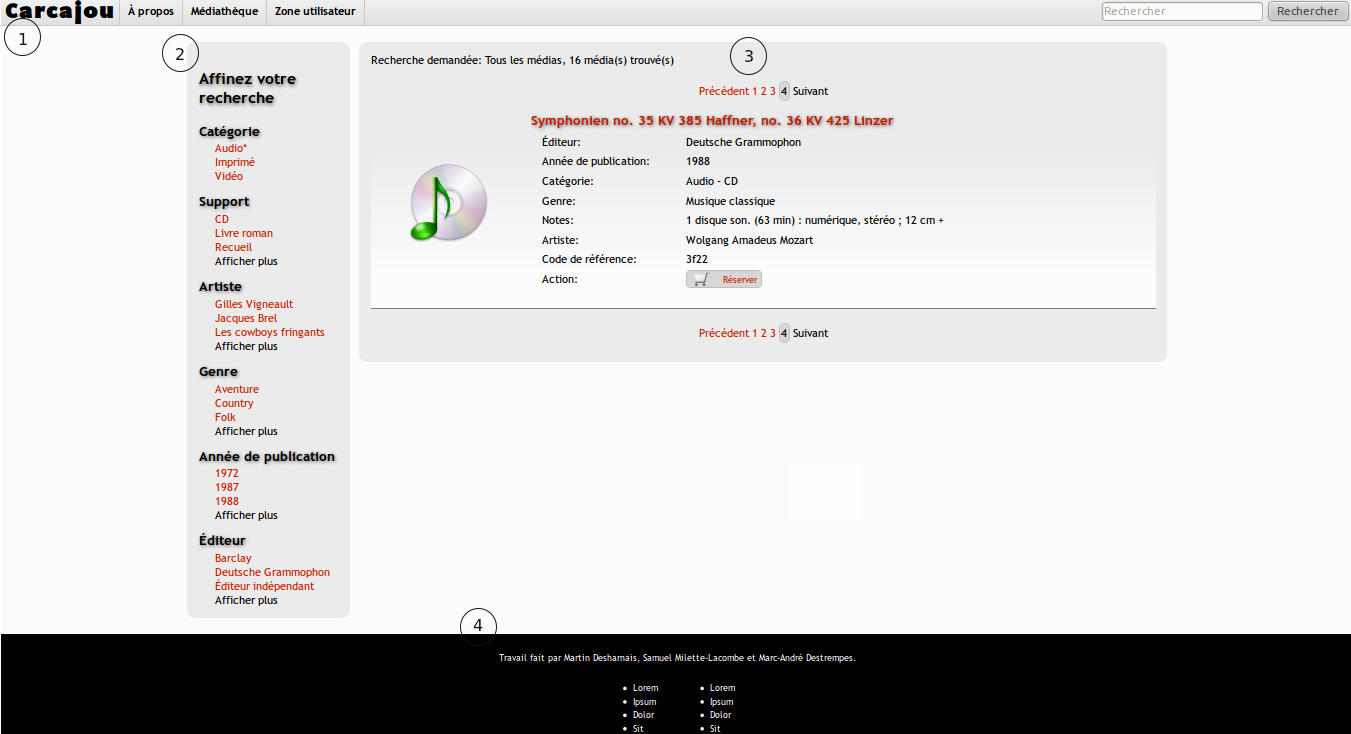
\includegraphics[scale=0.3]{pageType.png}
	\end{center}
	\caption{Exemple de page comprenant tous les éléments de la maquette}
\end{figure}

\subsection{Charte graphique}

\subsubsection{Couleurs}
La charte de couleur choisie est composée principalement de noir, de blanc et de différentes teintes de gris.

\begin{table}[h!tpb]
	\caption{Couleurs utilisées dans l'en-tête}
	\begin{center}
		\begin{tabular}{|l|l|l|}
			\hline
			Element      & Code     & Apercu \\
			\hline
			background 1 & \#FFFFFF & \cellcolor[HTML]{FFFFFF} \\ \hline
			background 2 & \#F5F5F5 & \cellcolor[HTML]{F5F5F5} \\ \hline
			background 3 & \#E3E3E3 & \cellcolor[HTML]{E3E3E3} \\ \hline
			border       & \#CCCCCC & \cellcolor[HTML]{CCCCCC} \\ \hline
			text         & \#000000 & \cellcolor[HTML]{000000} \\ \hline
			a            & \#000000 & \cellcolor[HTML]{000000} \\ \hline
		\end{tabular}
	\end{center}
\end{table}

\begin{table}[h!tpb]
	\caption{Couleurs utilisées dans le corps de la page}
	\begin{center}
		\begin{tabular}{|l|l|l|}
			\hline
			Element    & Code     & Apercu \\
			\hline
			background & \#000000 & \cellcolor[HTML]{000000} \\ \hline
			text       & \#FFFFFF & \cellcolor[HTML]{FFFFFF} \\ \hline
			a          & \#FFFFFF & \cellcolor[HTML]{FFFFFF} \\ \hline
		\end{tabular}
	\end{center}
\end{table}

\begin{table}[h!tpb]
	\caption{Couleurs utilisées dans le pied de page}
	\begin{center}
		\begin{tabular}{|l|l|l|}
			\hline
			Element      & Code     & Apercu \\
			\hline
			background 1 & \#FFFFFF & \cellcolor[HTML]{FFFFFF} \\ \hline
			background 2 & \#EEEEEE & \cellcolor[HTML]{EEEEEE} \\ \hline
			background 3 & \#DBD9D9 & \cellcolor[HTML]{DBD9D9} \\ \hline
			border 1     & \#C1C1C1 & \cellcolor[HTML]{C1C1C1} \\ \hline
			border 2     & \#C0C0C0 & \cellcolor[HTML]{C0C0C0} \\ \hline
			text         & \#000000 & \cellcolor[HTML]{000000} \\ \hline
			a            & \#C52100 & \cellcolor[HTML]{C52100} \\ \hline
		\end{tabular}
	\end{center}
\end{table}

\subsection{Typographie}

\subsubsection{Police d’écriture}

La police de caractère que nous avons choisi pour le site est Optima. Conformément à la convention, nous avons défini une liste de polices alternatives qui seront utilisées si la police Optima n'est pas disponible. La liste est, par ordre de priorité~: Trebuchet MS, Lucida, Arial, Geneva, Verdana, Lucida Grande, Tahoma, Helvetica, sans-serif.

Nous avons décidé de ne pas donner une taille fixe à la police de caractère, mais plutôt d'utiliser la taille désirée par l'utilisateur, définie dans les propriétés de son navigateur. Par exemple, pour configurer la taille de police par défaut sous Mozilla Firefox, il suffit d'aller dans \texttt{Préférences > Contenu > Polices et couleurs > Taille} et de définir la taille souhaitée. Nous sommes partis du principe que, si l'utilisateur a choisi d'afficher ses sites Internet avec une certaine taille, ce n'est pas à nous de contrevenir à sa volonté.

Cette taille définie par le navigateur est la taille par défaut d'un \texttt{em}. La taille de police par défaut du site est donc de \texttt{1em}.

\subsubsection{Titres}
Les titres sont de la même police de caractère que le reste du site, mais ont une taille plus importante, variant selon l'importance du titre.

\begin{table}[h!tbp]
	\caption{Taille des différents niveaux de titre}
	\begin{center}
		\begin{tabular}{|c|l|}
			\hline
			Titre & Taille \\
			\hline
			h1    & 1.9em\\
			h2    & 1.75em\\
			h3    & 1.4em\\
			h4    & 1.2em\\
			h5    & 1.15em\\
			h5    & 1.1em\\
			\hline
		\end{tabular}
	\end{center}
\end{table}

\subsubsection{Majuscules-minuscules}

Tous les titres commencent par une majuscule suivie par des minuscules. Il en est de même pour tout le texte contenu dans la page, c'est à dire, les paragraphes, les liens, etc.

\subsubsection{Arborescense du site}

Voir le diagramme en annexe.

\subsubsection{Images}

\begin{table}[h!tbp]
	\caption{Images}
	\begin{center}
		\begin{tabular}{|c|l|p{10cm}|}
		\hline
		Image                                            & Taille           & Description \\ \hline
		
\includegraphics[scale=0.2]{black_arrow_big.png} & 370x216, 209x122 & Cette image servira a afficher les détails d'un média sous forme d'infobulle.\\ \hline
		
\includegraphics{cart.png}                       & 20x20            & Icone représentant la réservation d'un média. \\ \hline
		
\includegraphics[scale=1.15]{emprunt.png}        & 87x87            & Icone représentant un emprunt. \\ \hline
		
\includegraphics[scale=0.3]{reservation.png}     & 87x87            & Icone représentant une réservation. \\ \hline
		
\includegraphics[scale=0.3]{audio.png}           & 128x128          & Logo signifiant la présence d'un média sous le format audio. \\ \hline
		
\includegraphics[scale=0.3]{imprime.png}         & 128x128          & Logo signifiant la présence d'un média sous le format imprimé. \\ \hline
		
\includegraphics[scale=0.3]{video.png}           & 128x128          & Logo signifiant la présence d'un média sous le format vidéo. \\ \hline
		
\includegraphics[scale=0.15]{search.png}         & 16x16            & Icone indiquant une recherche. \\ \hline
		
\includegraphics{down.png}                       & 21x4             & Indique que la colonne est triée par ordre croissant. \\ \hline
		
\includegraphics{up.png}                         & 21x4             & Indique que la colonne est triée par ordre décroissant. \\ \hline
		
\includegraphics{upAndDown.png}                  & 21x9             & Indique que la colonne n'est pas utilisée pour le tri. \\ \hline
		\end{tabular}
	\end{center}
\end{table}

\section{Modèle des pages principales et secondaires}

Dans l'idée de garantir une identité visuelle, toutes les pages du site sont construites sur une structure identique.

En tout, 7 modèles de pages ont été développés.

\begin{itemize}
	\item Le modèle de page descriptif;
	\item Le modèle d'affichage des résultats de recherche;
	\item Le modèle de page de réservations et emprunts;
	\item Le modèle tables de pilotage;
	\item Le modèle formulaire simple;
	\item Le modèle de détails avancé d'un média;
	\item Le modèle rapport.
\end{itemize}

\subsection{Le modèle de page descriptif}

Ce modèle est utilisé pour des pages d'information statiques. La page « À propos de la médiathèque » est un exemple de ce type de page. Les éléments que l'on retrouve dans ce modèle sont assez élémentaires. On y retrouve habituellement un titre de niveau 2, des paragraphes et une ou plusieurs images.

\begin{figure}[htbp]
	\begin{center}
		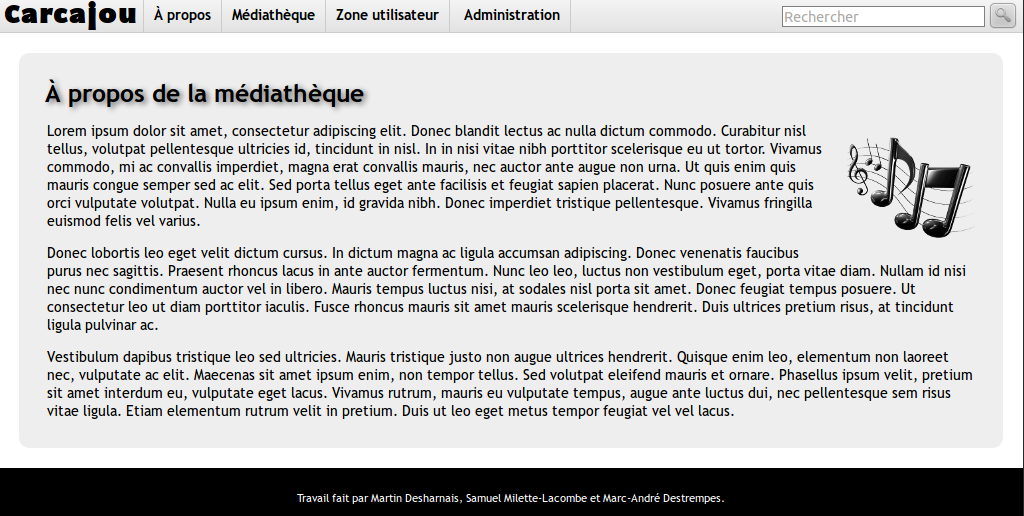
\includegraphics[scale=0.4]{captures_ecran/modele_descriptif.png}
	\end{center}
	\caption{Modèle descriptif}
\end{figure}

\subsection{Le modèle de page d'affichage des résultats de recherche}

Ce modèle est utilisé pour l'affichage des résultats de recherche. Il est considéré comme le type de page le plus fourni en terme de contenu. Il se compose des éléments suivants:

\begin{itemize}
	\item Un fil d'Ariane vertical disposé sur le côté gauche;
	\item Une description de la recherche en cours en haut de page;
	\item Le système de pagination en haut et en bas de la page;
	\item Les résultats de recherche sous forme d'élément de tableau contenant, les valeurs des champs standards à tous les médias, accompagnés d'une image.
\end{itemize}

\begin{figure}[htbp]
	\begin{center}
		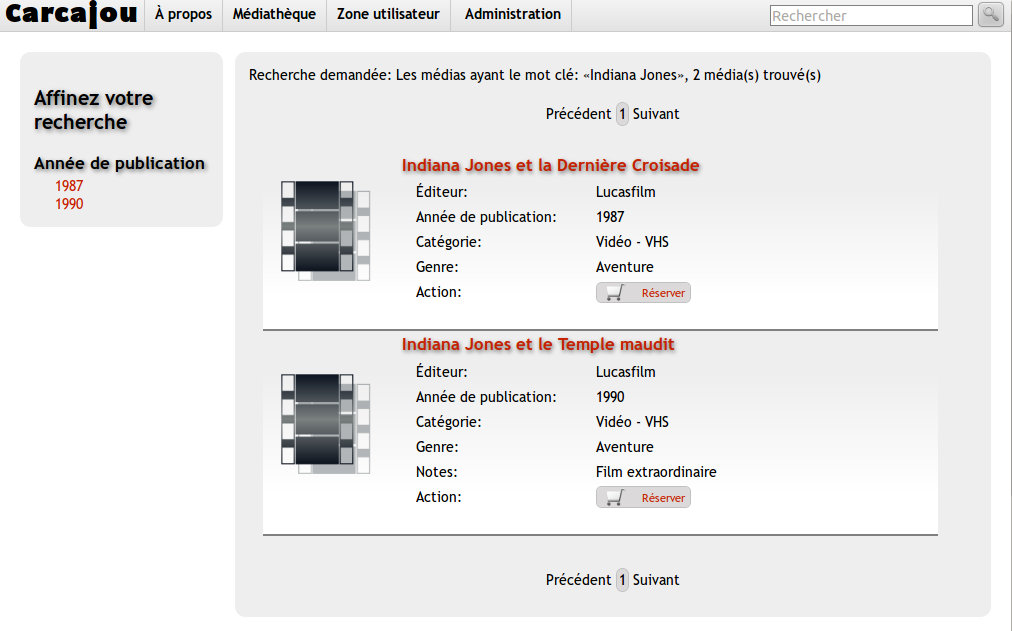
\includegraphics[scale=0.4]{captures_ecran/modele_resultats_recherche.png}
	\end{center}
	\caption{Modèle d'affichage des résultats de recherche}
\end{figure}

\subsection{Le modèle de page des réservations, des retours et des emprunts}

Ces modèles sont utilisés pour les pages de réservations, retours et d'emprunts. 

Pour la page de réservations, le média sélectionné est affiché avec ces détails, comme dans la recherche. Juste en dessous du média, l'utilisateur choisit s'il veut obtenir le média lorsqu'il sera disponible ou bien il choisit la plage de dates sur laquelle il veut réserver le média. Le bouton enregistrer envoie la réservation au serveur.

\begin{figure}[htbp]
	\begin{center}
		
\includegraphics[scale=0.4]{captures_ecran/reservation.png}
	\end{center}
	\caption{Modèle de réservations}
\end{figure}

Pour la page de retours, le matricule de l'utilisateur est entré à la main ou à l'aide du code QR. Le champ no. référence permet, soit à la main ou à l'aide du code QR d'ajouter ou bien de supprimer les médias. Le bouton enregistrer envoie le retour au serveur.

\begin{figure}[htbp]
	\begin{center}
		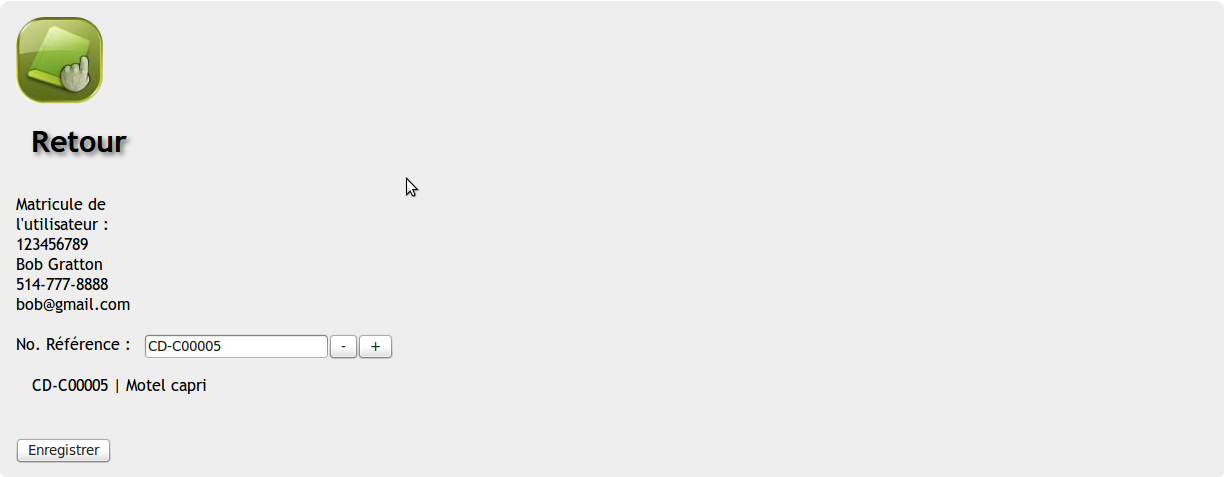
\includegraphics[scale=0.5]{captures_ecran/retour.png}
	\end{center}
	\caption{Modèle de retours}
\end{figure}

Pour la page d'emprunts, le modèle est exactement le même que celui des retours excepté le choix d'une plage de date sur laquelle le média sera emprunté.

\begin{figure}[htbp]
	\begin{center}
		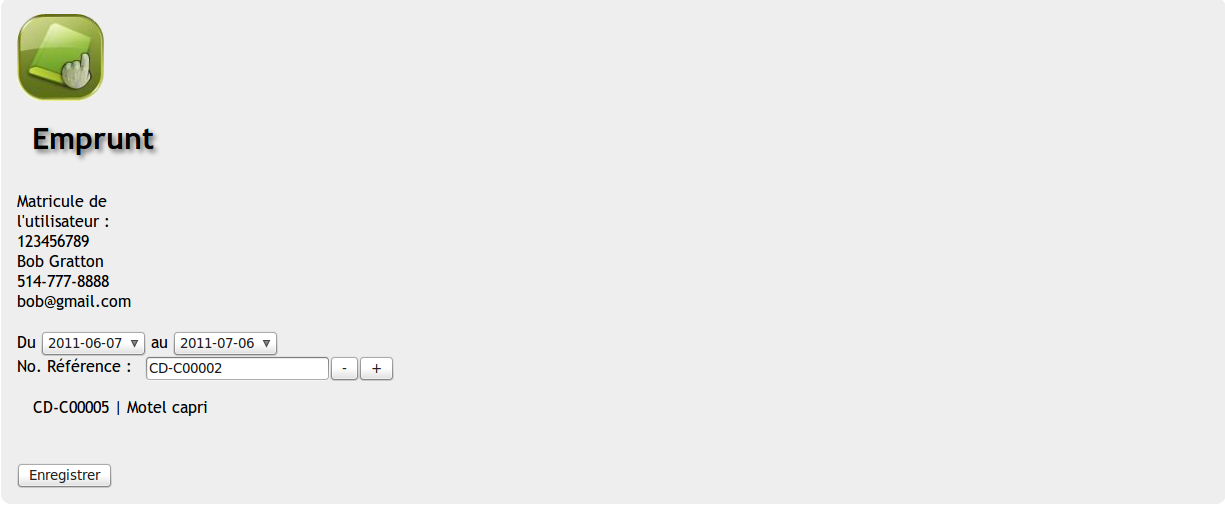
\includegraphics[scale=0.5]{captures_ecran/emprunt.png}
	\end{center}
	\caption{Modèle d'emprunts}
\end{figure}

\subsection{Le modèle de page table de pilotage}

Ce modèle est utilisé pour gérer le contenu des tables de pilotage\footnote{Voir la section \ref{sec:tables_de_pilotage} sur les tables de pilotage, à la page \pageref{sec:tables_de_pilotage}, pour plus de détails.}.

\begin{figure}[htbp]
	\begin{center}
		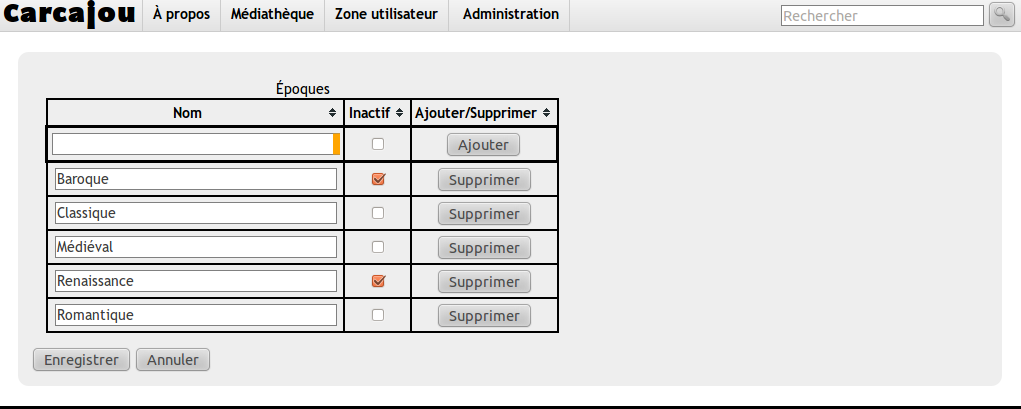
\includegraphics[scale=0.7]{captures_ecran/modele_tables_de_pilotage.png}
	\end{center}
	\caption{Modèle table de pilotage}
\end{figure}

\subsection{Le modèle de page formulaire simple}

Ce modèle est utilisé pour afficher des formulaires simples ayant un seul niveau de détail. Les éléments se retrouvant dans ce modèle sont constitués de quelques champs avec un bouton "Submit" permettant d'effectuer une action particulière sur les données. La page «~Suggestions~» en est un exemple.

\begin{figure}[htbp]
	\begin{center}
		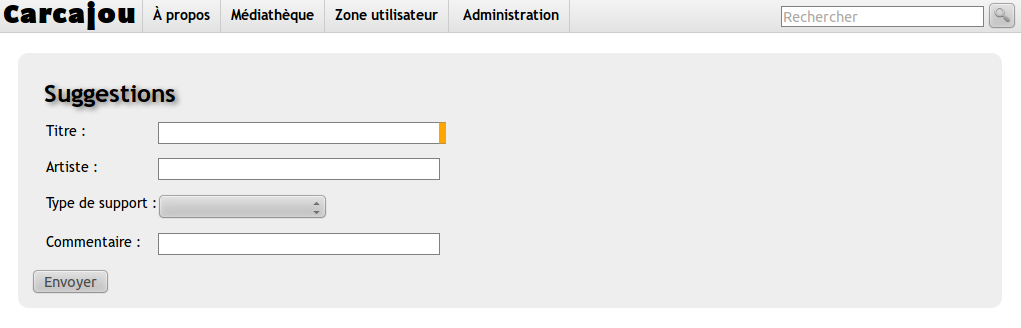
\includegraphics[scale=0.4]{captures_ecran/modele_formulaire_simple.png}
	\end{center}
	\caption{Modèle formulaire simple}
\end{figure}

\subsection{Le modèle de page de détails avancé d'un média}

Ce modèle est utilisé pour visionner ou modifier les détails d'un média. Lorsque l'utilisateur est un administrateur, les attributs des médias sont éditables sous forme de champs texte ou liste de sélection. On y retrouve des champs texte pour les champs indépendants des tables de pilotage et des listes de sélection lorsque ce sont des données provenant des tables de pilotage. Il existe plusieurs niveaux de détails pour un média. Le premier représente le média lui-même, comme un CD de musique, le second représente les enfants du médias, comme les différentes pistes de notre CD, alors que le troisième niveau représente les enfants du second niveau, tel que les différents artistes ayant participés à une piste. 

Puisque la quantité totale d'informations peut-être importante, tous les niveaux sont cachés par défaut et un résumé est affiché en lieu et place. Un clique sur le résumé fait apparaître l'enregistrement correspondant. De plus, des boutons plus et moins permettent d'ajouter et de supprimer des enregistrements des différents niveaux.

C'est là l'une des râres pages entièrement dépendante du JavaScript. Sans lui, il serait simplement impossible d'offrir la modification de tous les niveaux d'un média en une seule page.

Lorsque l'utilisateur n'est pas un administrateur, tous les champs éditables deviennent des éléments affichés.

\begin{figure}[htbp]
	\begin{center}
		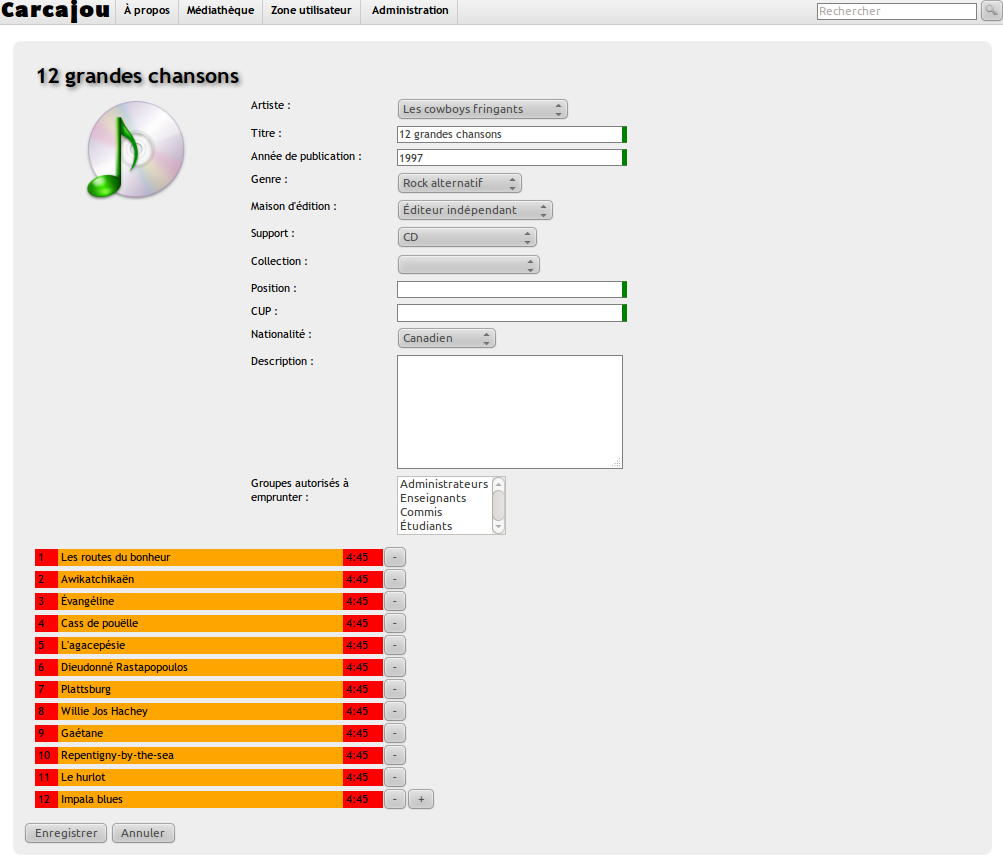
\includegraphics[scale=0.4]{captures_ecran/modele_details_medias.png}
	\end{center}
	\caption{Modèle formulaire simple}
\end{figure}

\subsection{Le modèle de page rapport}

Ce modèle de page est utilisé pour des données sous forme de rapports. Les rapports sont tout simplement constitués d'un tableau présentant les valeurs des différentes colonnes de la table dans la base de données.

\section{Diagramme d'enchaînement}

Voir le diagramme en annexe.

Pour accéder au niveau 2 du diagramme, nous devons emprunter exactement le chemin indiqué dans le schéma. Le niveau inférieur peut, en tout temps, accéder aux pages du niveau supérieur. Lors d'une connexion, si l'utilisateur n'est pas un administrateur nous ne lui affichons pas les pages emprunt et retour. Sinon, nous lui rajoutons ces options dans le menu.

\section{Diagramme de classe}

Voir l'API du système fourni avec le document.

\section{Base de données et dictionnaire}

Voir le tableau en annexe.

%%%%%%%%%%%%%%%%%%%%%%%%%%%%%%%%%%%%%%%%%%%%%%%%%%
\chapter{Architecture technologique}
%%%%%%%%%%%%%%%%%%%%%%%%%%%%%%%%%%%%%%%%%%%%%%%%%%

\section{Représentation graphique}

\begin{figure}[htbp]
	\begin{center}
		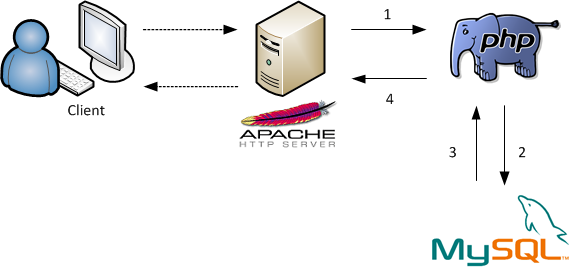
\includegraphics[scale=0.75]{architectureTechnologique.png}
	\end{center}
	\caption{Diagramme de l'architecture technologique}
\end{figure}

\section{Spécifications techniques}


\subsection{Navigateurs}
Lors de la conception, le site a été testé sur les navigateurs suivants~:

\begin{itemize}
	\item Mozilla Firefox 3.5.16
	\item Mozilla Firefox 3.6.10
	\item Mozilla Firefox 4.0.1
	\item Google Chrome 6.0.472.63
	\item Google Chrome 11.0.696.65
\end{itemize}

Le site est fonctionnel sur l'ensemble des navigateurs, mais certains effets graphiques ne sont disponibles que sur les versions récentes de chacun.

\subsection{Languages}
\subsubsection{Client}
Du côté client, les langages utilisés sont le HTML 5, le CSS 3, le JavaScript et le XML.

Pour le HTML 5 et le CSS 3, il a été décidé d'utiliser les fonctionnalités dont nous avions besoin tout en gardant en tête que le site devait rester consultable sur les navigateurs ne reconnaissant pas ces nouvelles technologies. Par exemple, la propriété CSS 3 «~border-radius~» nous permet d'afficher des coins arrondis facilement sur n'importe quel composant de la page. Dans le cas où celle-ci ne serait pas reconnue par un navigateur, celui-ci doit ignorera simplement la propriété et affichera des coins carrés standards.

Pour le JavaScript, la bibliothèque \href{http://jquery.com/}{jQuery 1.6.1} a été utilisée afin de simplifier le code et d'unifier la gestion des différents navigateurs. En effet, cette bibliothèque a l'avantage de proposer des fonctions unifiées qui se chargent pour nous de gérer les différences entre les différents navigateurs.

Cependant, il a été décidé de réduire au maximum la dépendance au JavaScript. Dans le cas de fonctionnalités JavaScript facultatives, comme le fait de n'afficher que les trois premiers éléments des listes trop longues, le code HTML ne contient qu'une liste toute simple et c'est au chargement de la page par le navigateur que le JavaScript s'occupe de modifier la structure du document et d'offre un bouton permettant d'afficher les éléments excédentaires.

Bien sûr, il y certains cas où le JavaScript est absolument obligatoire, comme la création de nouveaux champs dans les formulaires devant traiter un nombre variable d'enregistrements. Heureusement, ces cas complexes ne s'appliquent que dans des sections d'administration. Un visiteur ou un utilisateur disposant de droits minimaux peut donc se passer aisément de JavaScript et le site reste parfaitement consultable.

Pour le XML, celui-ci est utilisé comme moyen de transmission de l'information lors des requêtes AJAX. À l'heure actuelle, les requêtes AJAX sont faites à des fichiers XML statiques, mais, à terme, des scripts PHP devrons être écrits permettant de générer dynamiquement le fichier selon les critères reçus en paramètre.

\subsubsection{Serveur}
Du côté serveur, le seul langage utilisé est le PHP, qui a été utilisé dans ses versions 5.3.3 et 5.3.5 dépendamment des contributeurs.

Les conventions php utilisés sont les suivantes~:

\begin{itemize}
	\item Les fichiers contenant la définition d'une classe PHP utilisent l'extension «~.class.php~».
	\item Les fichiers contenant du code PHP qui doit obligatoirement être inclus dans un autre script utilisent l'extension «~.inc.php~».
	\item Les fichiers contenant du code PHP qui se suffit à lui-même utilisent l'extension «~.php~».
	\item Les fichiers contenant les pages finales affichées à l'utilisateur sont situés à la racine du projet (/).
	\item Les fichiers contenant des scripts PHP qui effectuent une action avant de rediriger l'utilisateur sont situés dans le répertoire php (/php/).
\end{itemize}

\subsection{Bande passante}
L'utilisation de la bande passante à été un sujet soins constants. La charte graphique du site se base massivement sur le CSS et n'utilise qu'un nombre très restreint d'images. De plus, la plupart des script JavaScript et codes CSS ont été placés dans des fichiers externes afin de bénéficier du cache des navigateur.

La page la plus lourde répertoriée (dûe à la présence de trois grosses images JPG) ne pèse que 139 kilo-octets, dont environ 40 ko peuvent être mis en cache, alors que la page d'accueil du site internet du cégep de Trois-Rivières en pèse 625\footnote{Il est à noter que, dans les deux cas, les chiffres donnés sont ceux donnés avec compression des données. Nous prenons pour acquis que la fonctionnalité sera activée sur le serveur web.}. La consommation de bande passante à donc été réduite au minimum et un forfait d'entrée de gamme se révèlera plus que suffisant afin de pourvenir aux besoins de la médiathèque.

\subsection{Serveurs}
Apache HTTP Server 2.2.16 -- 2.2.17

\subsection{Type de base de données}
MySQL 5.1.49 -- 5.5.8

Pour utiliser la base de données, il faut créer l'utilisateur \texttt{website@localhost} avec le mot de passe \texttt{1234}.

\section{Sécurité}
\label{sec:sécurité}

\subsection{En théorie}

La gestion des droits fait appel au «~bit~bashing~», une technique qui consiste à donner une représentation binaire à chacun des droits et de ne stocker que la somme de ces droits dans la base de données. Ainsi, si nous avons les droits suivants de définis~:

\begin{itemize}
	\item \$application->rights['read'] = 0001
	\item \$application->rights['write'] = 0010
	\item \$application->rights['execute'] = 0100
\end{itemize}

et qu'un groupe A dispose des droits de lecture et d'écriture dans la section «~administration~», et qu'un groupe B dispose du droit de renouveler un prêt la table \texttt{droits\_groupes} contiendrait quelque chose comme ceci~:

\begin{table}[ht]
	\caption{groupes}
	\begin{center}
		\begin{tabular}{|c|l|l|}
			\hline
			ID & nom & inactif \\
			\hline
			1  & A   & FALSE \\
			2  & B   & FALSE \\
			\hline
		\end{tabular}
	\end{center}
\end{table}

\begin{table}[h!]
	\caption{droits\_groupes}
	\begin{center}
		\begin{tabular}{|c|l|c|l|}
			\hline
			ID & section                 & groupeID & droits \\
			\hline
			1  & administration          & 1        & 0011 \\
			2  & Renouveller un document & 1        & 0100 \\
			3  & Renouveller un document & 2        & 0100 \\
			\hline
		\end{tabular}
	\end{center}
\end{table}

Dans cet exemple, nous pouvons voir que le groupe A dispose des droits de lecture et d'écriture ($ 0001 + 0010 = 0011 $) sur la section «~administration~» et qu'il a le droit de renouveler des documents puisqu'il a le droit d'exécution (0100) sur «~Renouveller un document~».

Le groupe B, quant à lui, ne dispose que du droit de renouveler des documents. En effet, si aucune entrée ne correspond à un groupe pour une section donnée, il est supposé que le groupe en question n'a aucun droit sur cette section. Le fait de ne créer aucun enregistrement est strictement identique au fait de créer un enregistrement contenant les droits (0000).

\begin{table}[h!]
	\caption{utilisateurs}
	\begin{center}
		\begin{tabular}{|c|l|l|l|l|}
			\hline
			ID & matricule & nom         & prenom   & inactif \\
			\hline
			1  & 11111111  & Baggins     & Frodo    & FALSE \\
			2  & 22222222  & Gamgee      & Samwise  & FALSE \\
			3  & 33333333  & Brandybuck  & Meriadoc & TRUE \\
			4  & 44444444  & Took        & Peregrin & FALSE \\
			\hline
		\end{tabular}
	\end{center}
\end{table}

\begin{table}[h!]
	\caption{groupes}
	\begin{center}
		\begin{tabular}{|c|l|l|}
			\hline
			ID & nom               & inactif \\
			\hline
			1  & Administrateurs   & FALSE \\
			2  & Enseignants       & FALSE \\
			3  & Commis            & FALSE \\
			4  & Étudiants         & FALSE \\
			5  & Prêtre            & TRUE \\
			\hline
		\end{tabular}
	\end{center}
\end{table}

\begin{table}[h!]
	\caption{groupes\_utilisateurs}
	\begin{center}
		\begin{tabular}{|c|c|c|}
			\hline
			ID & exID & groupeID \\
			\hline
			1  & 1    & 1 \\
			2  & 2    & 4 \\
			3  & 2    & 3 \\
			4  & 3    & 4 \\
			5  & 4    & 2 \\
			\hline
		\end{tabular}
	\end{center}
\end{table}

\begin{table}[h!]
	\caption{droits\_groupes}
	\begin{center}
		\begin{tabular}{|c|l|c|c|}
			\hline
			ID & section                & groupeID & droits \\
			\hline
			1  & drivingTable.php       & 1        & 0011 \\
			2  & drivingTable.php       & 2        & 0001 \\
			3  & drivingTable.php       & 3        & 0001 \\
			4  & drivingTable.php       & 5        & 0001 \\
			5  & Renouveler un document & 1        & 0100 \\
			6  & Renouveler un document & 2        & 0100 \\
			7  & Renouveler un document & 3        & 0100 \\
			8  & Renouveler un document & 4        & 0100 \\
			9  & Renouveler un document & 5        & 0100 \\
			10 & Emprunter un document  & 1        & 0100 \\
			11 & Emprunter un document  & 2        & 0100 \\
			12 & Emprunter un document  & 3        & 0100 \\
			13 & Emprunter un document  & 5        & 0100 \\
			\hline
		\end{tabular}
	\end{center}
\end{table}

L'exemple précédant couvre la plupart des situations qui peuvent survenir.

La table \texttt{utilisateurs} nous informe qu'il y a quatre utilisateurs d'enregistrés dans le système, mais que l'un d'entre eux est inactif. Un utilisateur inactif perd automatiquement tous ses droits.

La table \texttt{groupes} nous informe qu'il y a cinq groupes d'enregistrés dans le système, mais que l'un d'entre eux est inactif. Un groupe inactif perd automatiquement tous ses droits et ne peut plus être assigné à de nouveaux utilisateurs.

La table \texttt{groupes\_utilisateurs} nous informe que l'utilisateur 1 (Frodo Baggins) fait partit du groupe \emph{Administrateurs}\footnote{Par convention, le groupe \emph{Administrateurs} dispose généralement de tous les droits sur le système.}, que l'utilisateur 2 (Samwise Gamgee) fait partit à la fois du groupe \emph{Étudiants} et du groupe \emph{Commis}, que l'utilisateur 3 (Meriadoc Brandybuck) fait partit du groupe \emph{Étudiants} et, finalement, que l'utilisateur 4 (Peregrin Took) fait partit du groupe \emph{Enseignants}.

Enfin, la table \texttt{droits\_groupes} nous informe si chaque groupe peut~:

\begin{itemize}
	\item Afficher ou modifier les résultats de la page drivingTable.php;
	\item Effectuer l'action de renouveler un document;
	\item Effectuer l'action d'emprunter un document.
\end{itemize}

Nous voyons ainsi que les commis et les enseignants ont accès à la page drivingTable.php en lecture seule et que les administrateurs y ont accès en lecture-écriture. Les prêtres auraient aussi eu accès en lecture seule, mais en désignant leur groupe comme inactif, ils ont perdu tous leurs droits; L'enregistrement numéro 4 doit donc être ignoré par le processus de traitement des droits. Les étudiants, quant à eux, n'ont aucun enregistrement correspondant à cette section. Il est alors présumé qu'ils n'ont aucun droit sur la page drivingTable.php.

Nous voyons que tous les groupes d'utilisateurs ont le droit de renouveler un document, mais, encore une fois, l'enregistrement concernant les prêtres doit être ignoré.

Nous voyons enfin que tous les groupes, à l'exception des étudiants, ont le droit d'effectuer un emprunt\footnote{Veuillez noter que c'est le fait d'entrer un nouvel emprunt dans le système qui est traité ici. En effet, un simple étudiant doit demander à un commis qui, lui, se chargera d'entrer son emprunt dans le système.}.

Les utilisateurs actifs disposent de la somme des droits de chacun de groupes actifs auxquels ils appartiennent. Ainsi, Samwise Gamgee, qui est à la fois un étudiant et un commis, gagne le droit de consulter la page drivingTable.php en lecture seule et d'entrer des emprunts dans le système alors que Perigrin Took, qui est inactif, n'a aucun droit sur le système, quels que soient les groupes auxquels il appartient.

\subsection{En pratique}
La sécurité repose essentiellement sur la validation des droits des utilisateurs lors de la génération des pages du site. C'est le PHP qui est responsable de valider que l'utilisateur courant dispose des droits suffisants avant d'ajouter une section à la page que le serveur HTTP s’apprête à retourner.

En pratique, cela se traduit par un appel à la fonction \$application->currentUser->haveRights() en lui spécifiant en premier paramètre la section dont on veut valider les droits et, en second paramètre, la liste des droits dont l'utilisateur doit disposer pour avoir accès à ce contenu. Ces droits sont définis dans le tableau \$application->rights. Par exemple afin de valider que l'utilisateur ait bien le droit d'accéder à la zone d'administration, il suffit d'utiliser le code suivant~:

\begin{lstlisting}[style=php]
if($application->currentUser->haveRights('administration', $application->rights['read'] | $application->rights['write']))
{
	// We can now print administration section
}
else
{
	// Current user does not have suffisent rights
}
\end{lstlisting}

Du point de vue de l'utilisateur de la fonction, c'est extrêmement simple. Pour celui qui devra l'implémenter, c'est une autre histoire. Plaçons-nous un peu à la place du programmeur. Nous sommes dans une fonction dont voici la signature~:

\begin{lstlisting}[style=php]
public function haveRights($section, $rights)
{
	// TODO: Implement function
}
\end{lstlisting}

Pour atteindre son but, il dispose des informations suivantes :

\begin{itemize}
	\item \$section qui est la section dont l'on veut tester les droits;
	\item \$rights qui sont les droits que l'on doit tester;
	\item \$application->currentUser retourne une instance de la classe User représentant l'utilisateur actuellement connecté;
	\item \$application->database retourne une instance de la classe PDO représentant la base de données;
	\item \$application->rights retourne un tableau associatif contenant la représentation numérique de tous droits.
\end{itemize}

Pour pouvoir déterminer si l'utilisateur courant a bien les droits demandés, il faudra exécuter une requête à la base de données qui nous retourne la liste de tous les droits qu'à cet utilisateur sur cette section\footnote{Il peut y en avoir plus d'un si l'utilisateur appartient à plus d'un groupe.}, additionner ces droits grâces à l'\href{http://www.php.net/manual/en/language.operators.bitwise.php}{opérateur «~ou~binaire~»} (binary or) et déterminer si tous les bits à 1 dans les droits demandés sont aussi à 1 dans les bits des droits de l'utilisateur grâce à l'opérateur «~et~binaire~» (binary and).

\subsection{En conclusion}
Cette façon de gérer les droits des utilisateurs offre de nombreux avantages~:

\begin{itemize}
	\item La plus grande partie de la gestion des droits est centralisée dans la base de données plutôt que de s'éparpiller dans de multiples fichiers;
	\item La notion de groupes permet de généraliser des droits semblables à de nombreux utilisateurs;
	\item Le fait qu'un utilisateur puisse appartenir à plusieurs groupes offre un haut niveau de granularité, tout en restant facultatif;
	\item Le fait qu'un groupe ne dispose que des droits explicitement définis assure la sécurité, car tout nouveau droit n'est effectif que pour ceux qui l'on explicitement reçus.
	\item L'utilisation du «~bit~bashing~» plutôt que des colonnes explicitement définies permet d'ajouter très facilement de nouveaux types de droits à ceux déjà définis (read, write, execute).
\end{itemize}

%%%%%%%%%%%%%%%%%%%%%%%%%%%%%%%%%%%%%%%%%%%%%%%%%%
\chapter{Prototype fonctionnel}
%%%%%%%%%%%%%%%%%%%%%%%%%%%%%%%%%%%%%%%%%%%%%%%%%%

\appendix

\chapter{Dictionnaire de données}
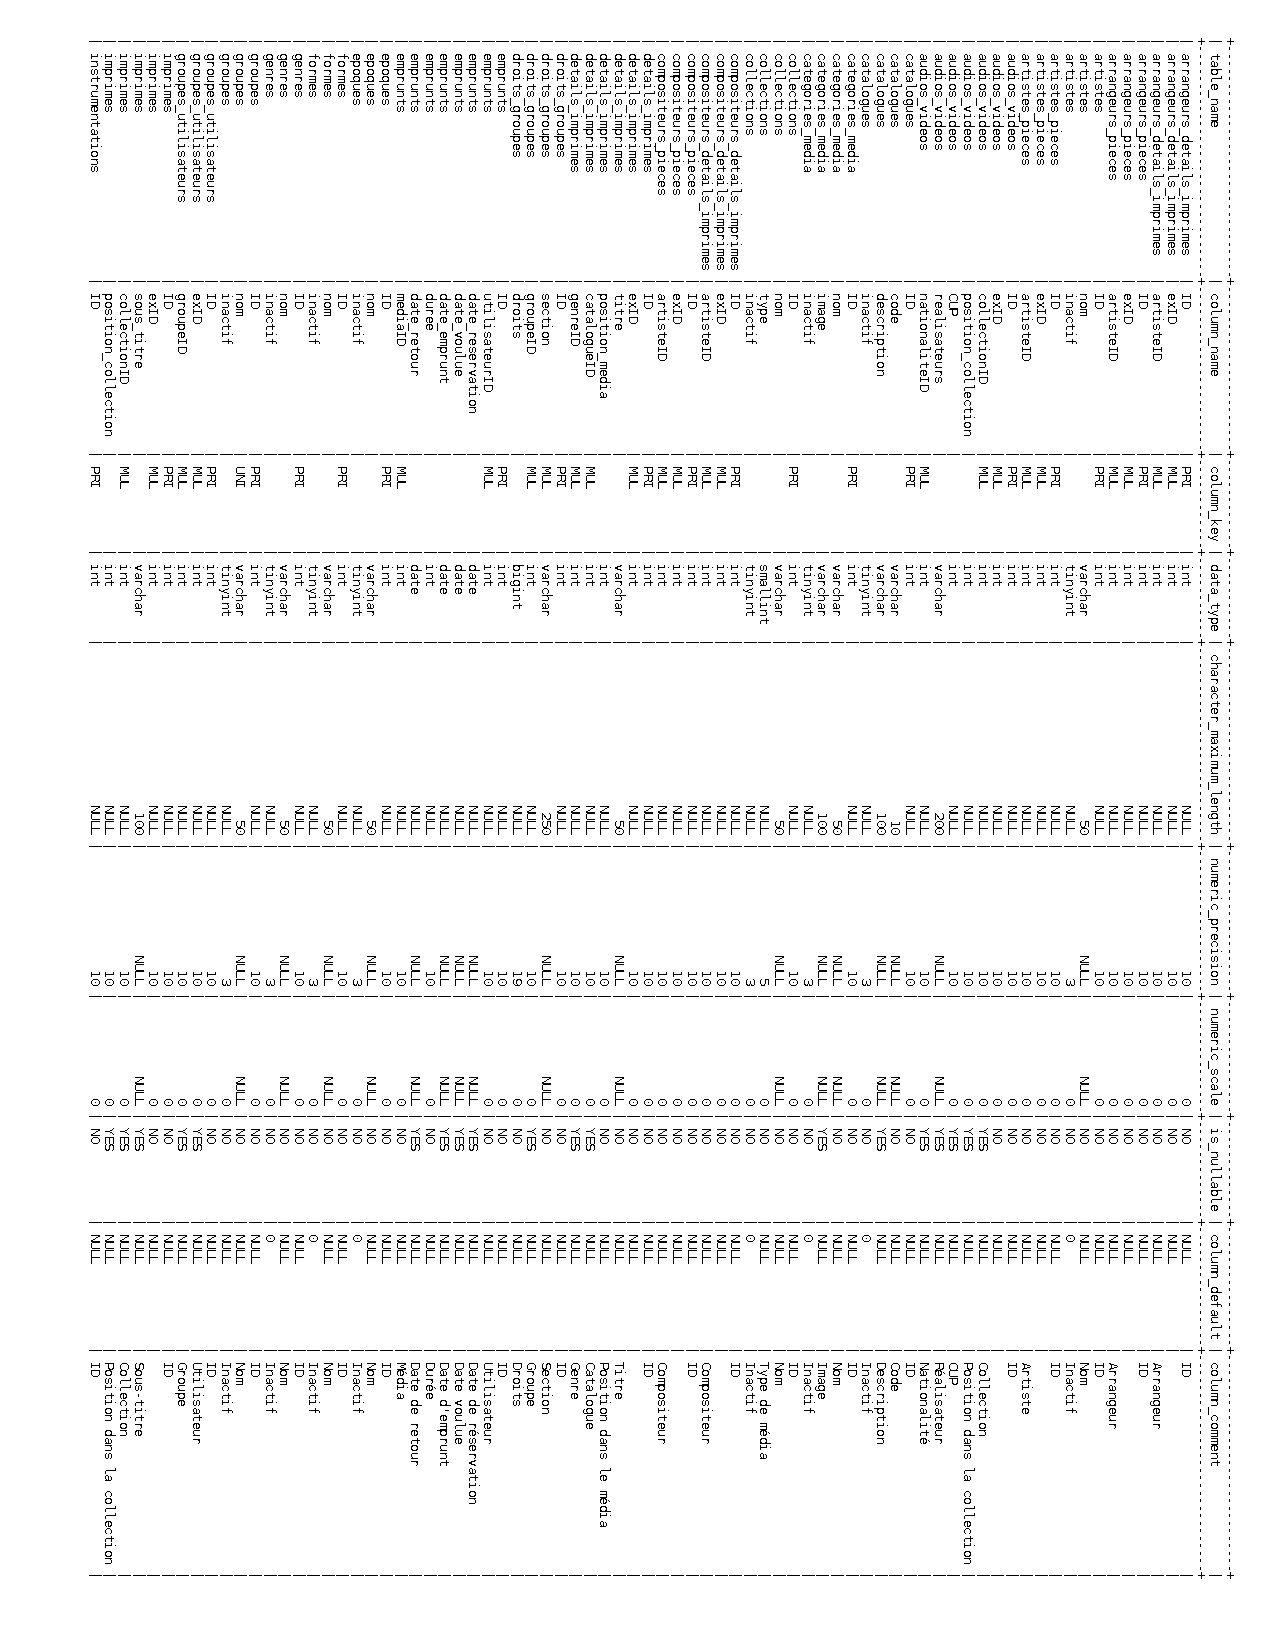
\includepdf[pages=-]{dataDictionary.pdf}

\chapter{Diagramme d'enchaînement}
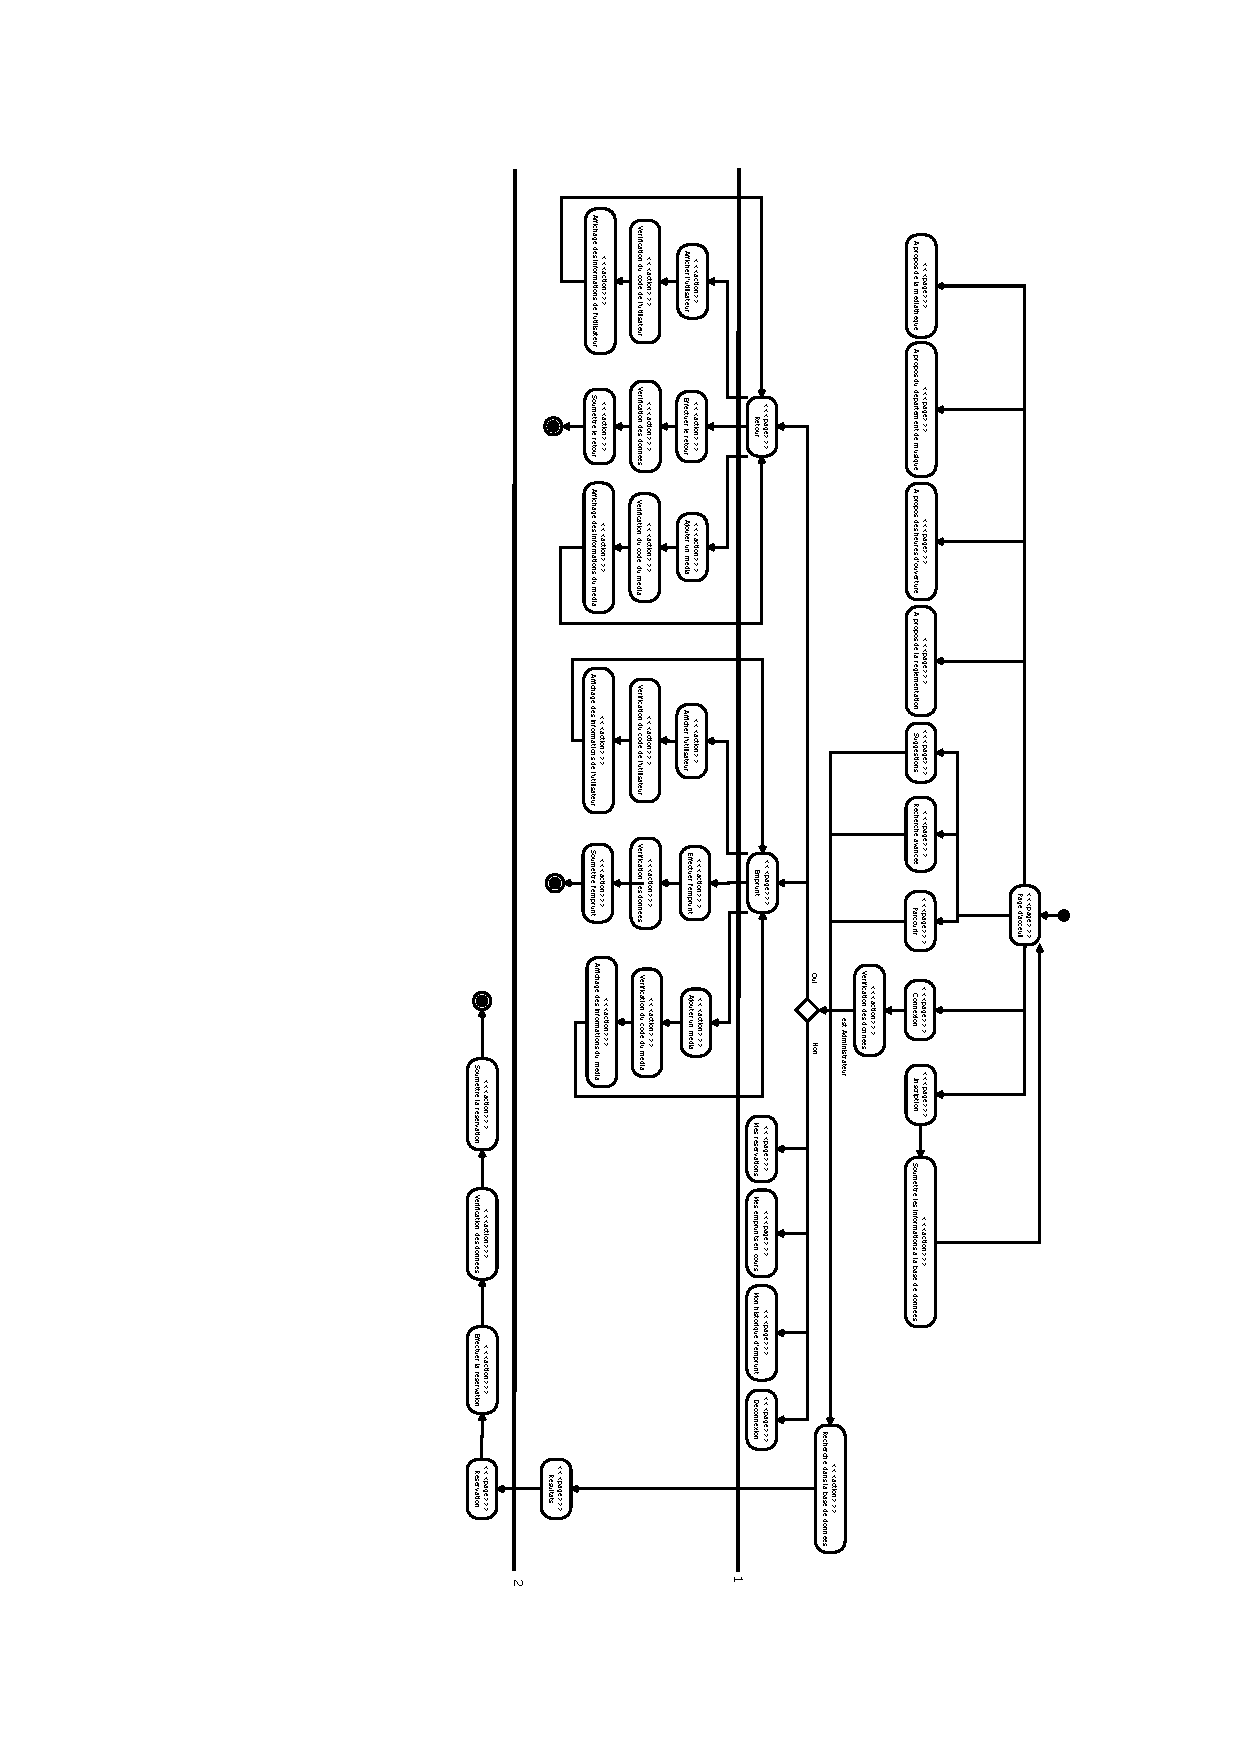
\includepdf[page=-]{diagrammeEnchainement.pdf}

\chapter{Arborescence du site}
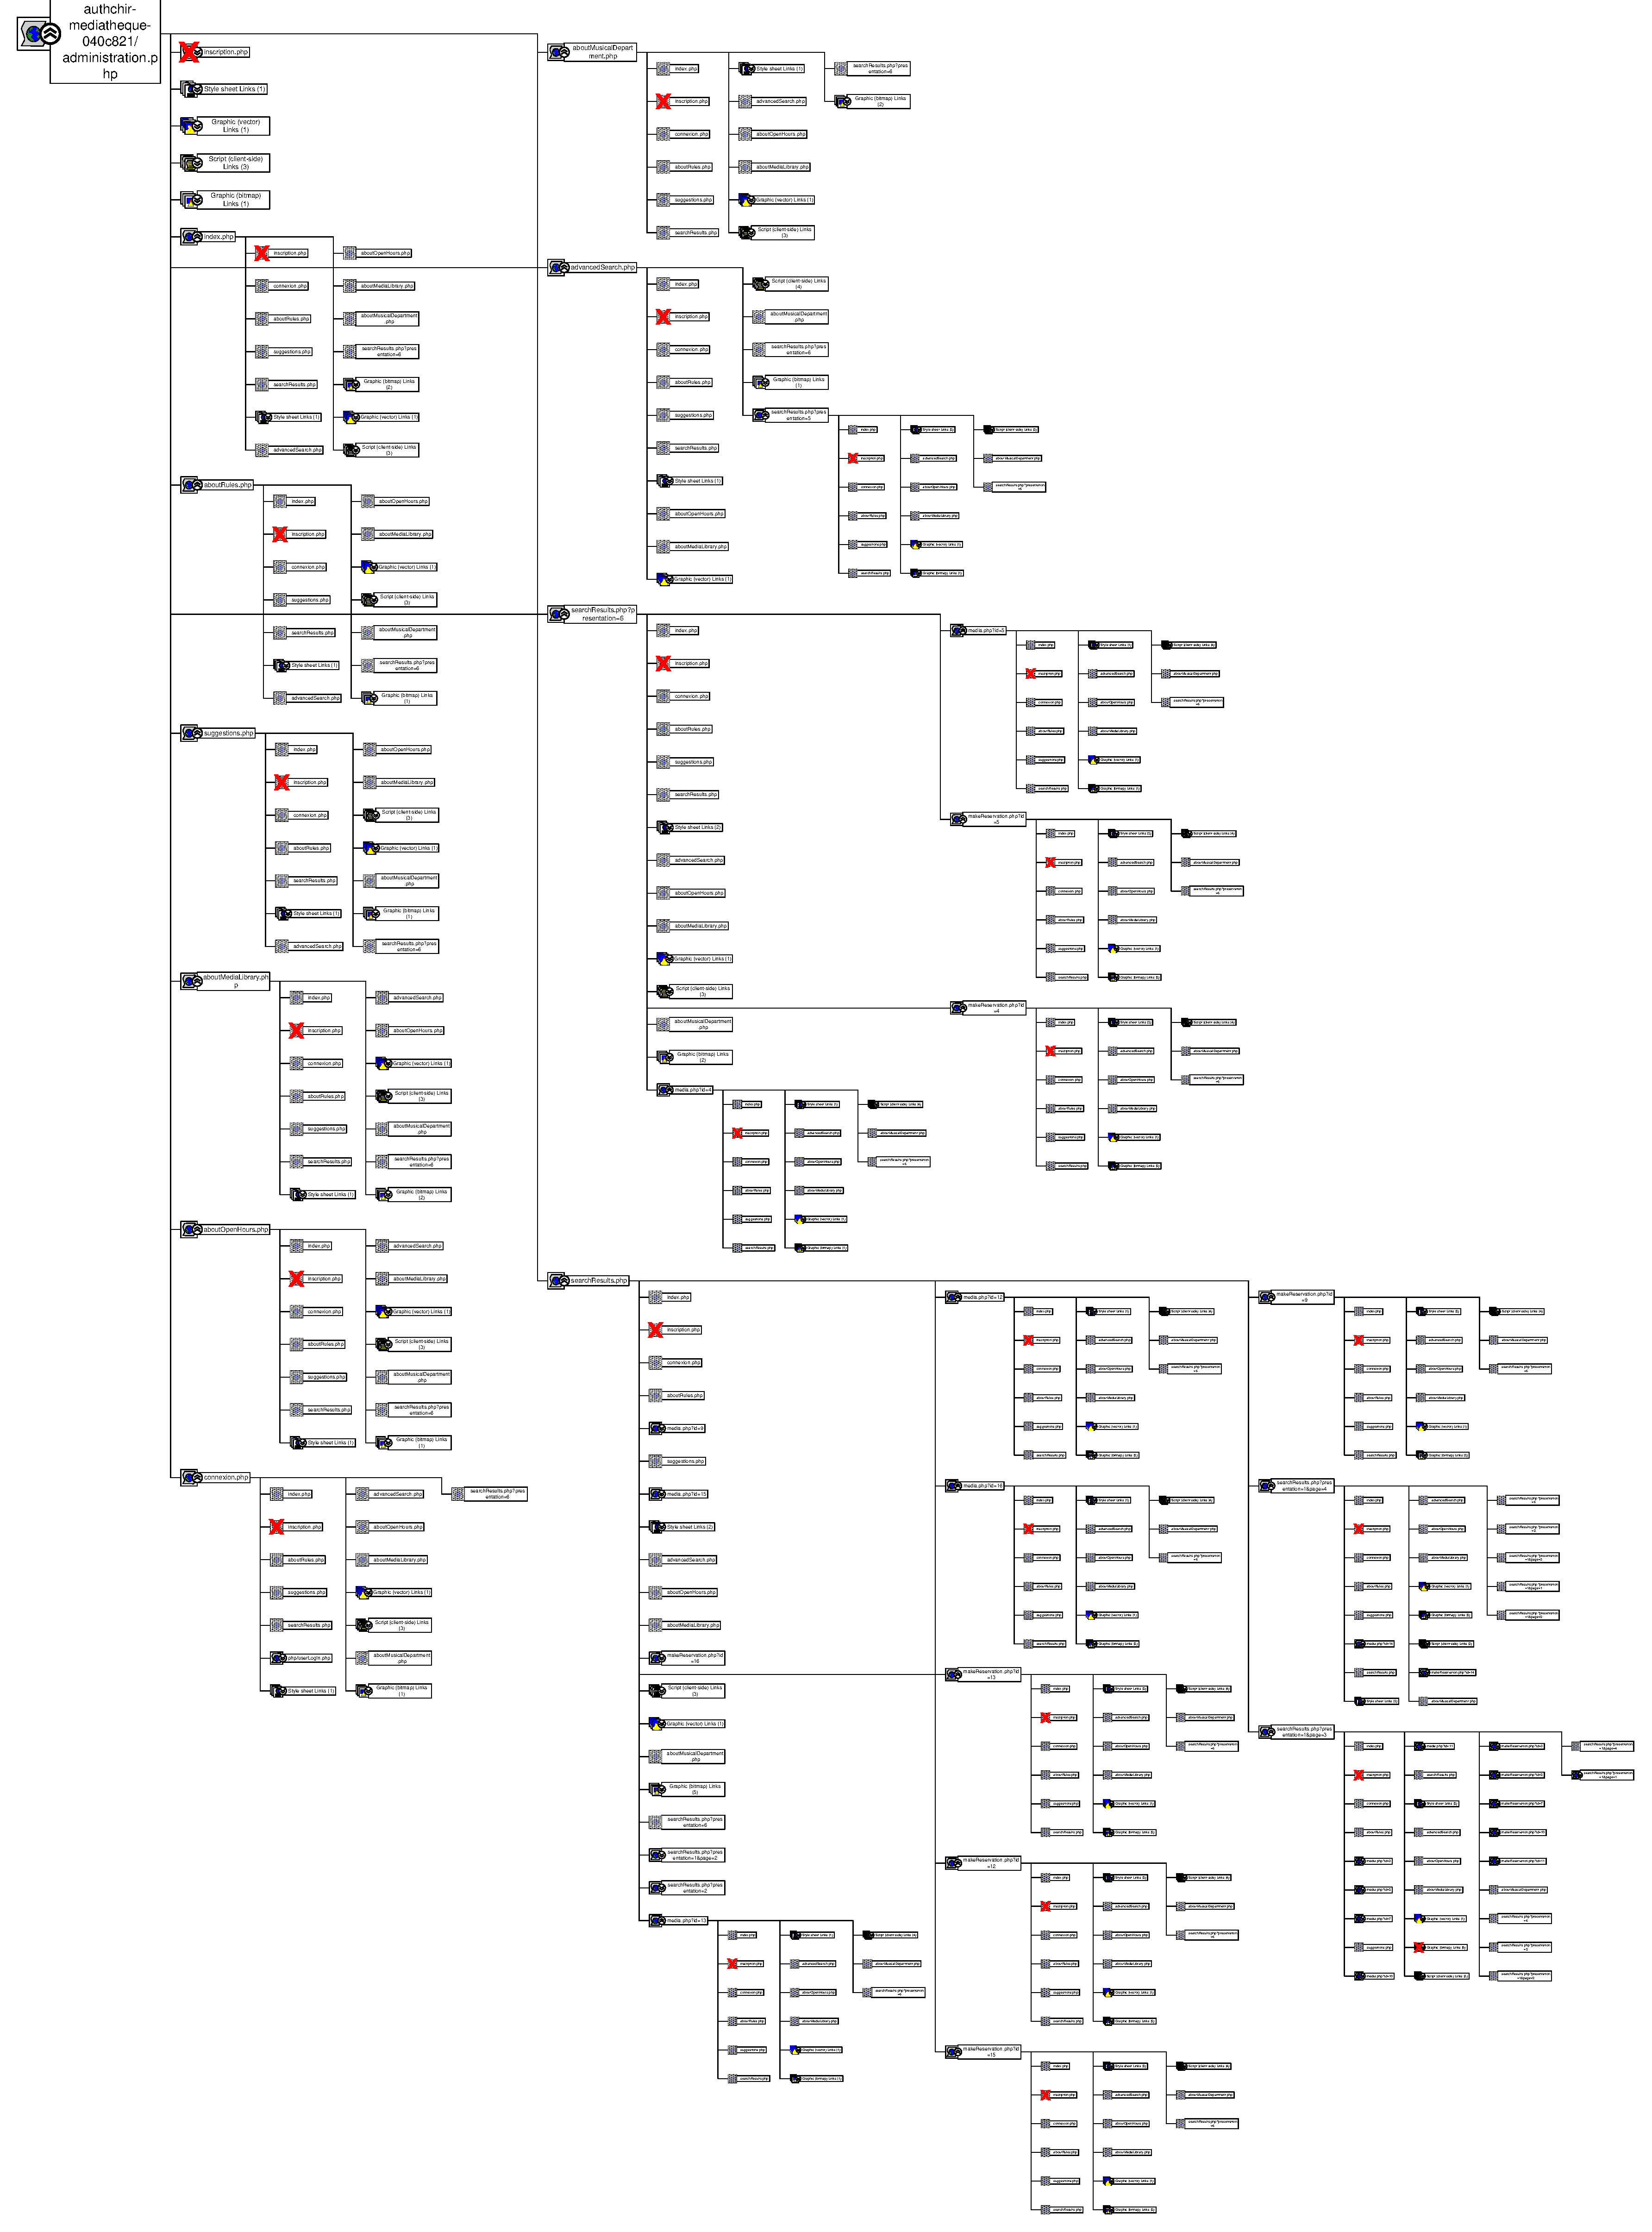
\includepdf[page=-]{arborescenceDuSite.pdf}

\listoffigures
\listoftables

\end{document}
